%\documentclass[a4paper,10pt,fleqn]{PhDthesisPSnPDF}
\documentclass[a4paper,10pt,fleqn]{report}
\usepackage{epsf}
\linespread{1.1}    
\usepackage{graphicx}
\usepackage{listings}
\usepackage{color}
\usepackage{multirow}
\usepackage{hyperr	ef}
\usepackage{float}
\restylefloat{table}
\usepackage[style=authoryear,backend=bibtex8]{biblatex}
\usepackage[tableposition=top]{caption}
\usepackage{usecases}
\addbibresource{0144266.bib}

\definecolor{dkgreen}{rgb}{0,0.6,0}
\definecolor{gray}{rgb}{0.5,0.5,0.5}
\definecolor{mauve}{rgb}{0.58,0,0.82}
\lstset{frame=tb,
  language=Java,
  aboveskip=3mm,
  belowskip=3mm,
  showstringspaces=false,
  columns=flexible,
  basicstyle={\small\ttfamily},
  numbers=left,
  numberstyle=\tiny\color{gray},
  keywordstyle=\color{blue},
  commentstyle=\color{dkgreen},
  stringstyle=\color{mauve},
  breaklines=true,
  breakatwhitespace=true
  tabsize=3
}

\setlength{\textheight}{8.5in}
\setlength{\oddsidemargin}{0.5in}
\setlength{\evensidemargin}{0.5in}
\setlength{\textwidth}{5.50in}
\setlength{\topmargin}{0.0in}
\setlength{\headheight}{0in}
\setlength{\headsep}{0in}
%\setlength{\parindent}{12mm}
% paragraph indent
\setlength{\parindent}{0pt}
% spacing between paragraphs
\setlength{\parskip}{1ex plus 0.5ex minus 0.2ex}


%\usepackage{thesis}
\pagestyle{plain}

\begin{document}
\title{Hibernate 'til Spring \\ Benefits of Spring MVC, Hibernate and Apache Tiles to Support Quality Attributes and Usability within Web Applications}
\author{Chris O'Brien}
%\date{}
\maketitle

\begin{abstract}      
Web development is one of the fastest growing areas in software development, with new tools being developed yearly. 








\end{abstract}        

%
% Table Of Contents
%
\tableofcontents

%
% List of figures
%
\listoffigures

%
% List of tables
%
\listoftables

\chapter{Introduction}
\label{intro}

\section{General Introduction}

This project concerns the development of a web application using a web framework in conjunction with a number of other tools. This project concerns the development of a web application using a web framework in conjunction with a number of other tools. Throughout development, there is a particular cognisance towards the support of Non-Functional Requirements (NFR) by both the web framework and the supporting tools throughout the development process.  The web application framework used within the project is Spring MVC and the Object Relational Mapping (ORM) framework Hibernate for data persistence. This project consists of both a software engineering component, in the shape of the web application developed using the tools discussed within this report, and a research component consisting of this report.

This project intends to discover any benefits, and limitations, that the use of a framework has in the development of a web application, and its non functional requirements. The scope of this project will focus on security, productivity, extensibility, usability and performance and the effect that the use of frameworks has on these attributes.

The application resulting from this project will be evaluated a number of ways. The Open Web Application Security Project (OWASP) Top 10 vulnerabilities are used to evaluate security within the application. Previous experience, specifically obtained from both \textit{Systems Architecture and Design} and \textit{Distributed Systems}, was used to guide evaluation of productivity and performance. These modules exposed this author to Message Passing Interfaces (MPI), the use of architectural patterns in order to support extensibility, and the concept of servlets within an web application, and the environment in which it runs. Examples in the Evaluation section are taken from the \textit{Distributed Systems} project, and show how security is implemented without the use of a framework. This is used to evaluate how these frameworks support productivity and performance. The usability study is a framework taken from \parencite{holzinger2005usability} and applied to the final application resulting from this FYP, and two other related web applications. 



\section{Technology}

The technology needed for a web application such as the one created for this FYP requires a certain architecture, shown in Figure~\ref{fig:webarch}. The application consists of three layers: Presentation, Business and Data. The application runs on an application server, namely Tomcat 7. Other alternatives are the open source Glassfish 4, and IBMs WebSphere. Tomcat 7 was chosen ahead of Glassfish as while Glassfish provides more utility in that it supports Enterprise Java Beans, these were not needed for this application. Tomcat 7 requires considerably less memory than Glassfish to operate, and will require less resources to run. 

\begin{figure}[H]
\begin{center}
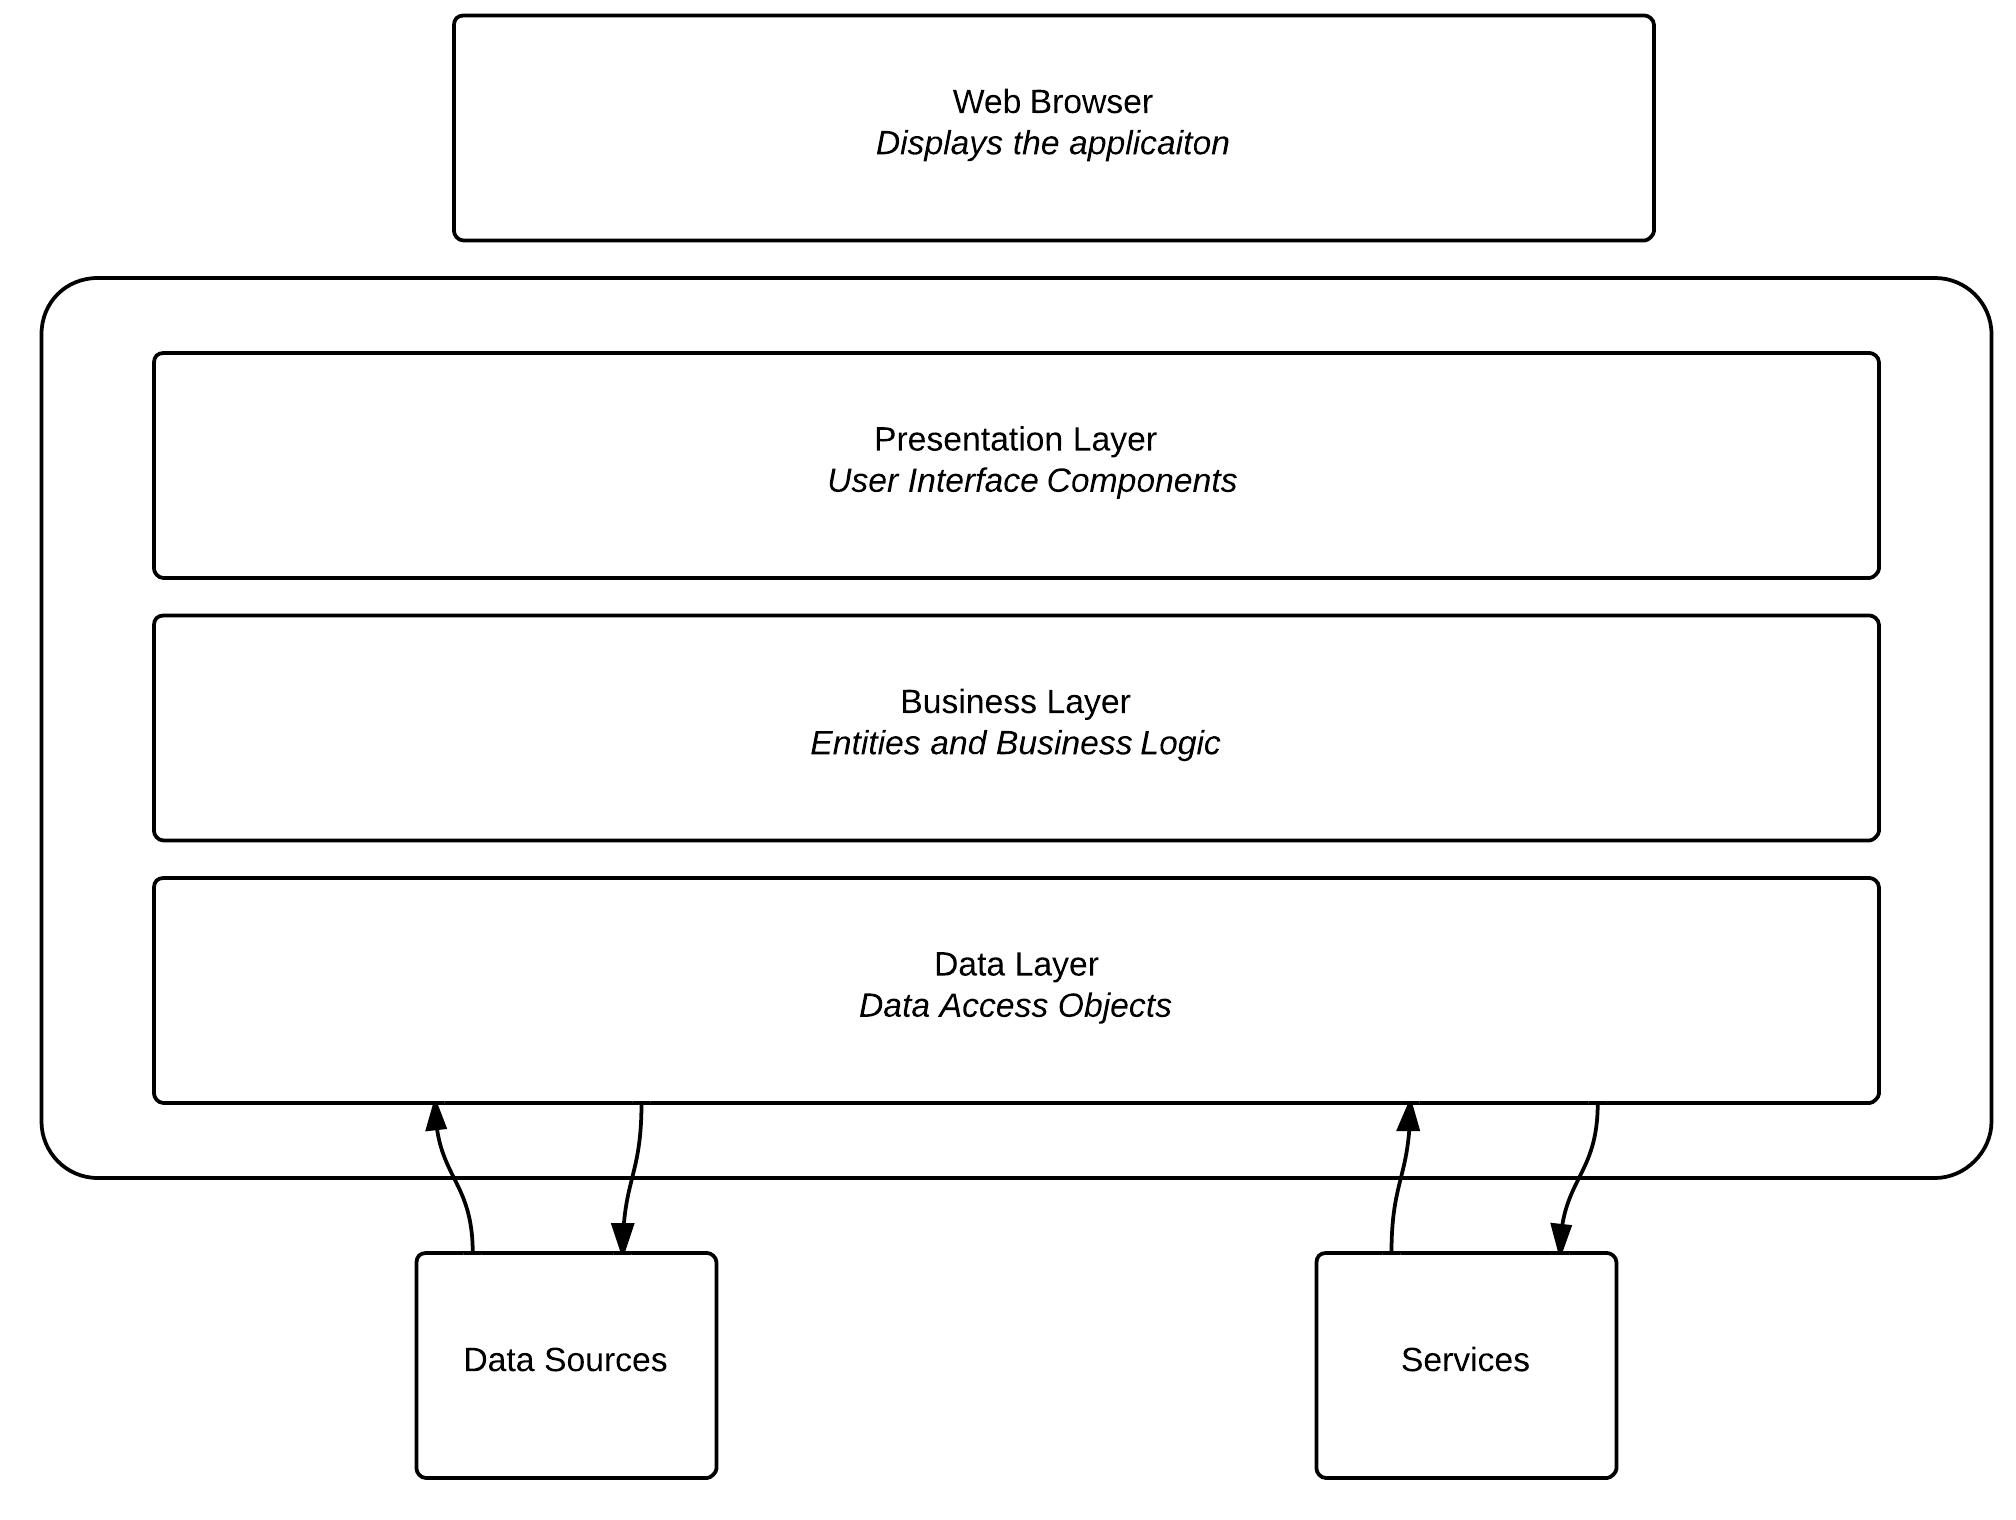
\includegraphics[scale=0.24]{webapp.PNG}
\end{center}
\caption{Typical architecture of a web application}
\label{fig:webarch}
\end{figure}

\begin{figure}[H]
\begin{center}
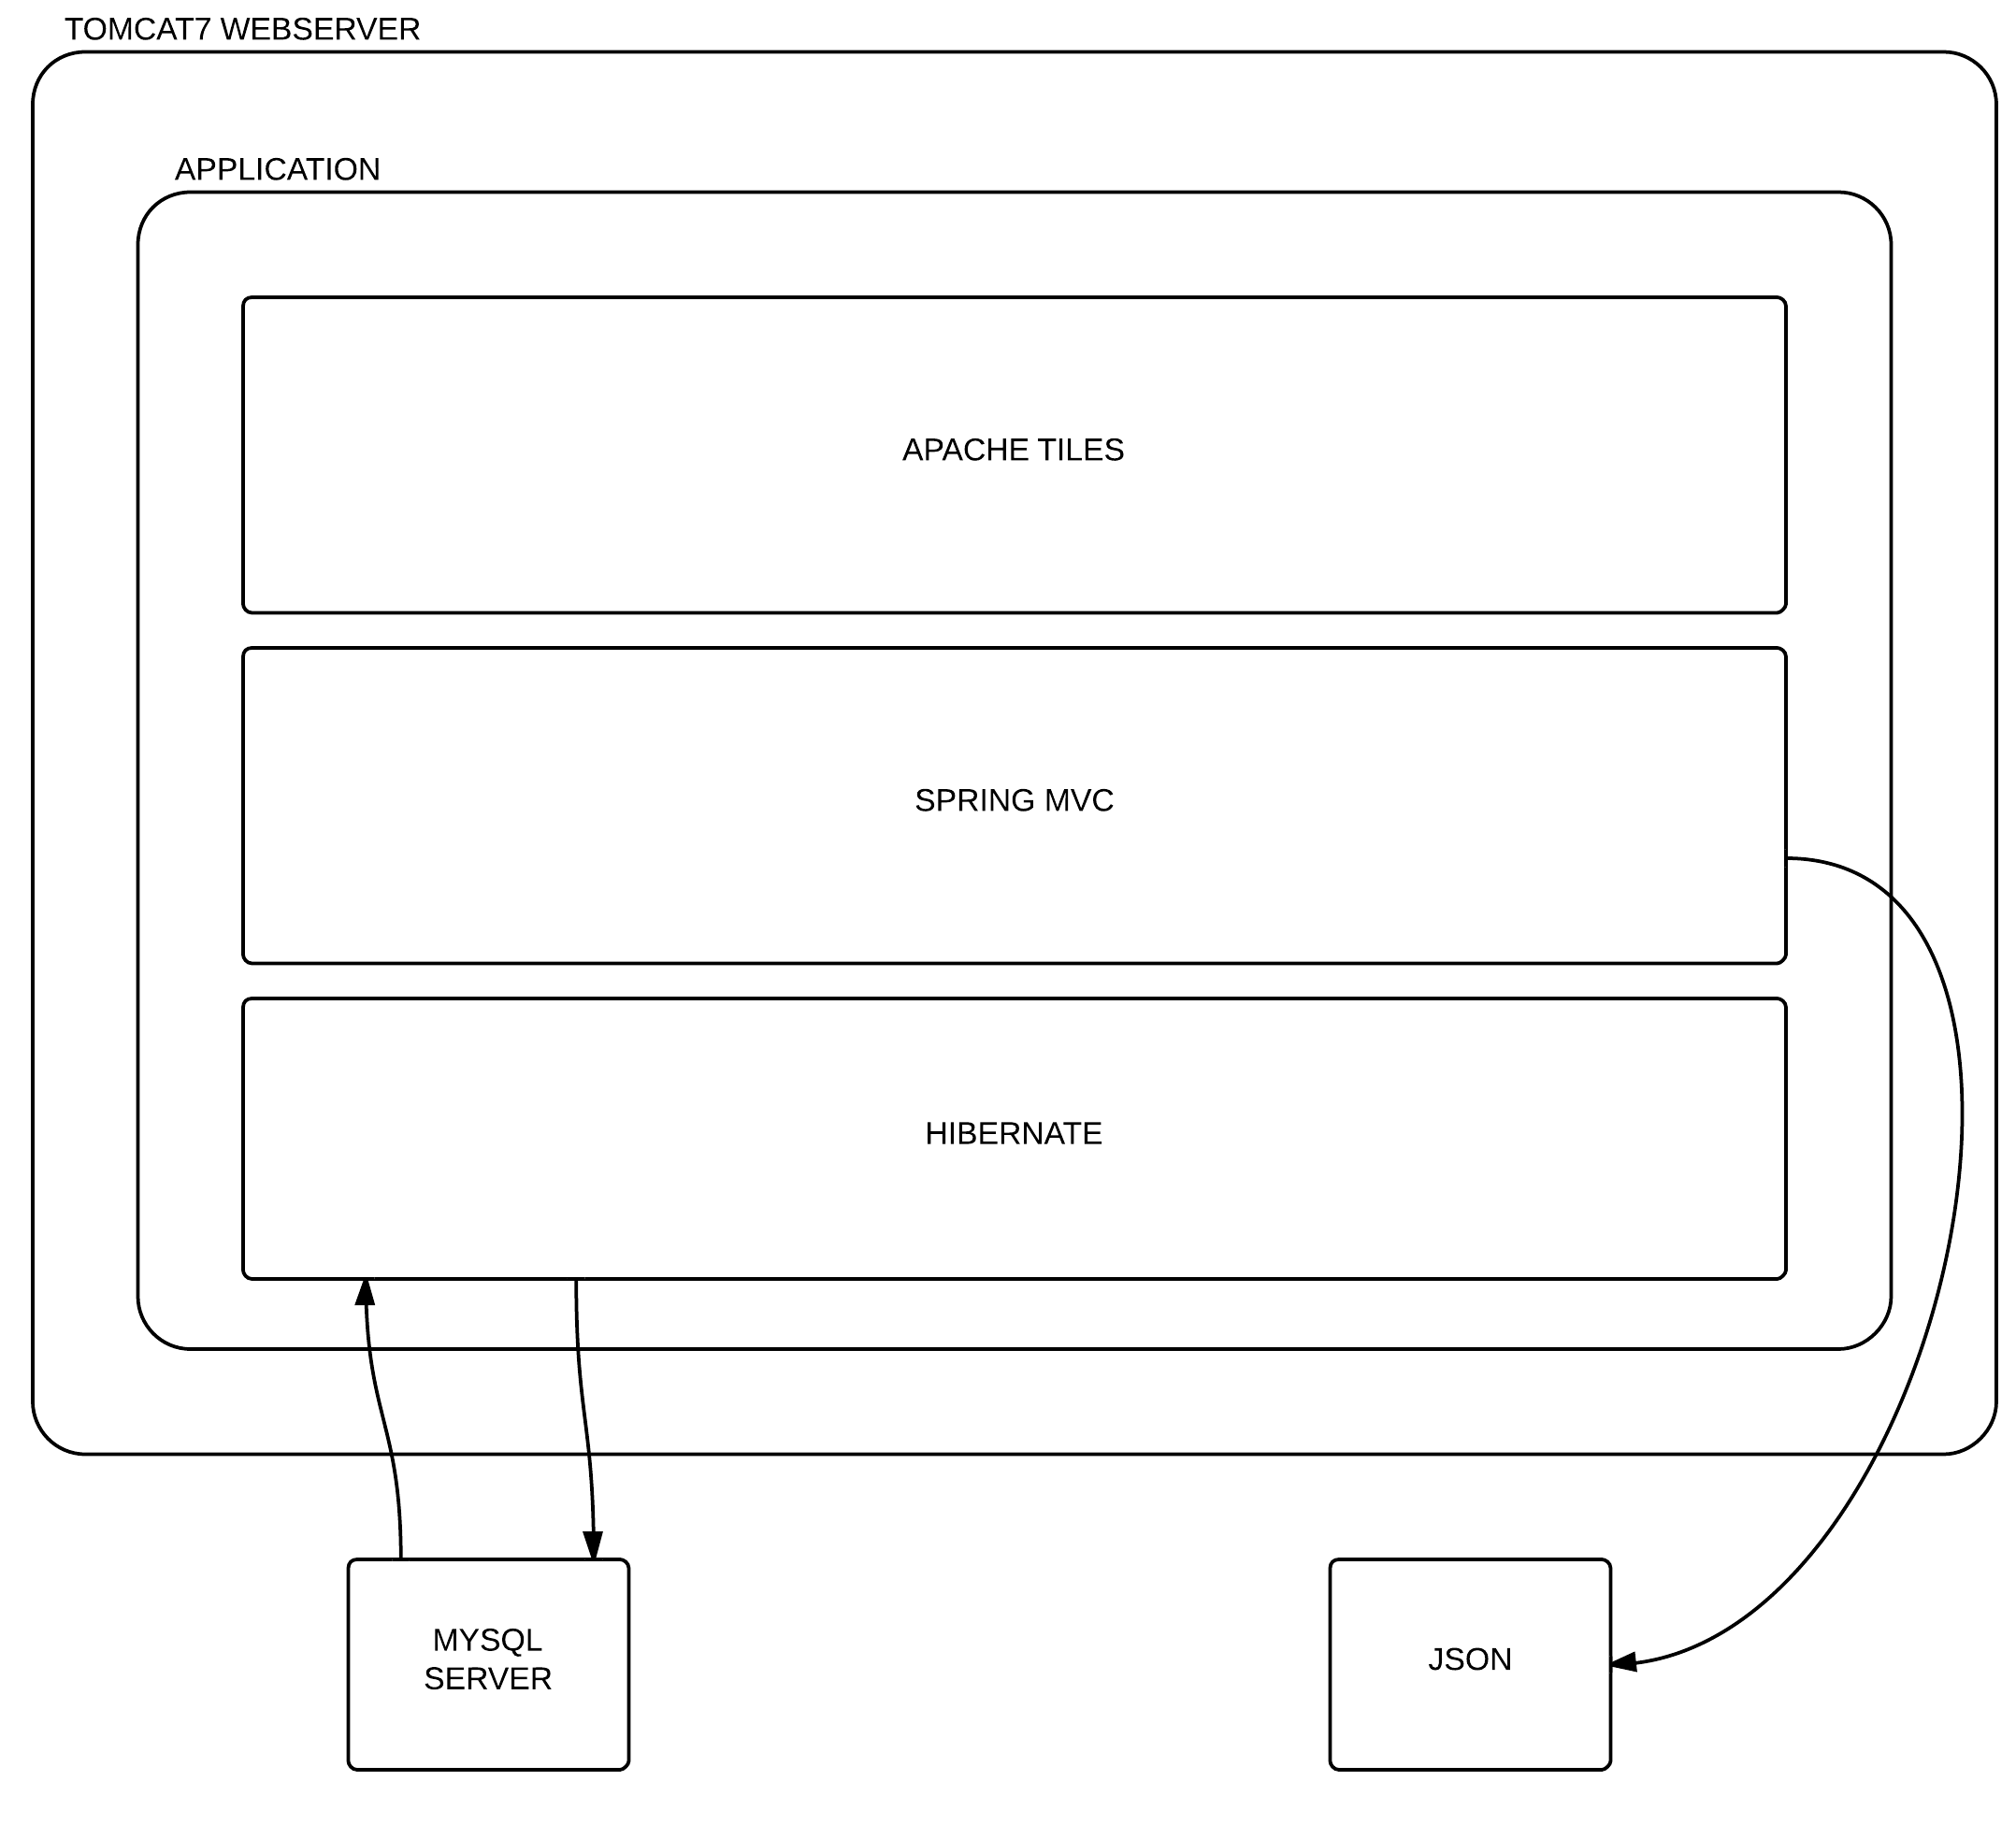
\includegraphics[scale=0.24]{projarch.PNG}
\end{center}
\caption{Architecture of FYP application}
\label{fig:projstack}
\end{figure}

\section{Objectives}

\subsection{Primary Objectives}

The primary objective of this project is to show the benefits to quality attributes that the use of an architectural stack provides. The architectural stack within this project contains Spring MVC, Hibernate ORM and Apache Tiles. 

This project will examine the support provided for specific quality attributes: Security, Productivity, Extensibility and Performance. The provision of these attributed as provided by these frameworks will be examined, with cognisance of usability. 

\subsection{Secondary Objectives}

The secondary objectives of this project are: 

\begin{itemize}
\item To gain knowledge of the development of a web application using frameworks
\item To obtain experience working with a architectural stack common to industry
\item To use metrics and code visualisations within a project in order to guide and aid development of an application.
\end{itemize}

\section{Scope}

This report, and project, are focused on the effect that frameworks have on quality attributes. As such, the full functionality of the web application is outside the scope of this project. While requirements are an important part of every software lifecycle process, the full methodology for requirements elicitation is outside the scope of this project. Though web services are touched on briefly, they, and mobile viewing, are not important to the overall project, and are not discussed. 

\section{Methodology}

The methodology used for this project was as follows

\begin{enumerate}
\item Learn the technology
\begin{itemize}
\item The first thing that was examined was the configuration of the technologies needed to implement a web application using Spring, Hibernate and Tiles. As such a set of tutorial videos provided by an educational website called Udemy provided a starting point. The paid videos totalled about 28 hours of content spread over 170 videos.\parencite{udemy}
\end{itemize}
\item Define objectives
\begin{itemize}
\item The next step was to define learning objectives from the project. The decision was made to focus on the support of specific quality attributes by the use of web application frameworks. This is the main objective of the paper, with secondary objectives relating to the use of metrics within a development in order to support overall quality of the application.
\end{itemize}
\item Requirements Engineering
\begin{itemize}
\item The elicitation of requirements from key stakeholders was an important step, and ensured that development of the application was in line with the expectations of those eventually utilising the application. Storyboarding, exploratory interviews and focus groups were used to elicit possible functional requirements, and to identify non function requirements key to the application.
\end{itemize}
\item Design
\begin{itemize}
\item The design of the system, such as the structure for user authentication, and the overall design of the application were examined, with cognisance of design patterns. The frameworks used within this application mandate programmers technique, and guide developers towards best practice.
\end{itemize}
\item Implementation, Testing and Deployment
\begin{itemize}
\item Once design of the application was completed, it needed to be implemented. Due to time constraints within a final year project, unit testing and some light user testing were the only techniques available to use. Deployment was a personal goal, as previous project had all been local applications.
\end{itemize}
\item Evaluation
\begin{itemize}
\item Evaluation of the application was performed by comparing the final application to previous work involving security completed in a previous module, Distributed Systems. OWASP was chosen to evaluate the security component of the application. Productivity was examined through a comparative use of both Hibernate and JDBC within one of the Data Access Object (DAO) classes. A performance test was prepared for comparing Hibernate and JDBC. A usability study, based on a framework \parencite{holzinger2005usability}, is also documented and a number of applications evaluated.
\end{itemize}
\end{enumerate}
\chapter{Background}
\label{background}

\section{Introduction}

There are a number of components needed to build the architecture of a web application. The nature of these components is explored below, and their contribution to the creation of a web application is analysed. A more detailed breakdown on their usage within the application is explored in subsequent chapters.

(bit about usability to go here)

\section{Technologies}

\subsection{Web Application Framework}
The Web Application Framework [WAF] chosen for this project is Spring MVC. Shan and Hua define a WAF as “a defined support structure in which other software applications can be organized and developed”. (Shan and Hua 2006). MVC, or Model-View-Controller, is a software pattern that facilitates the use of a user interface, shown in its classic form in Figure~\ref{fig:mvcclassic}. The intention of this pattern is to form a clear division between domain objects and presentation objects. The Model manages the behaviour and data of the application. The View manages the information obtained from the model and displays it to the user. The Controller manages user input, such as key strokes, mouse movements or a touch display, and can interact and invoke functionality within the Model and/or View.

\begin{figure}[H]
\begin{center}
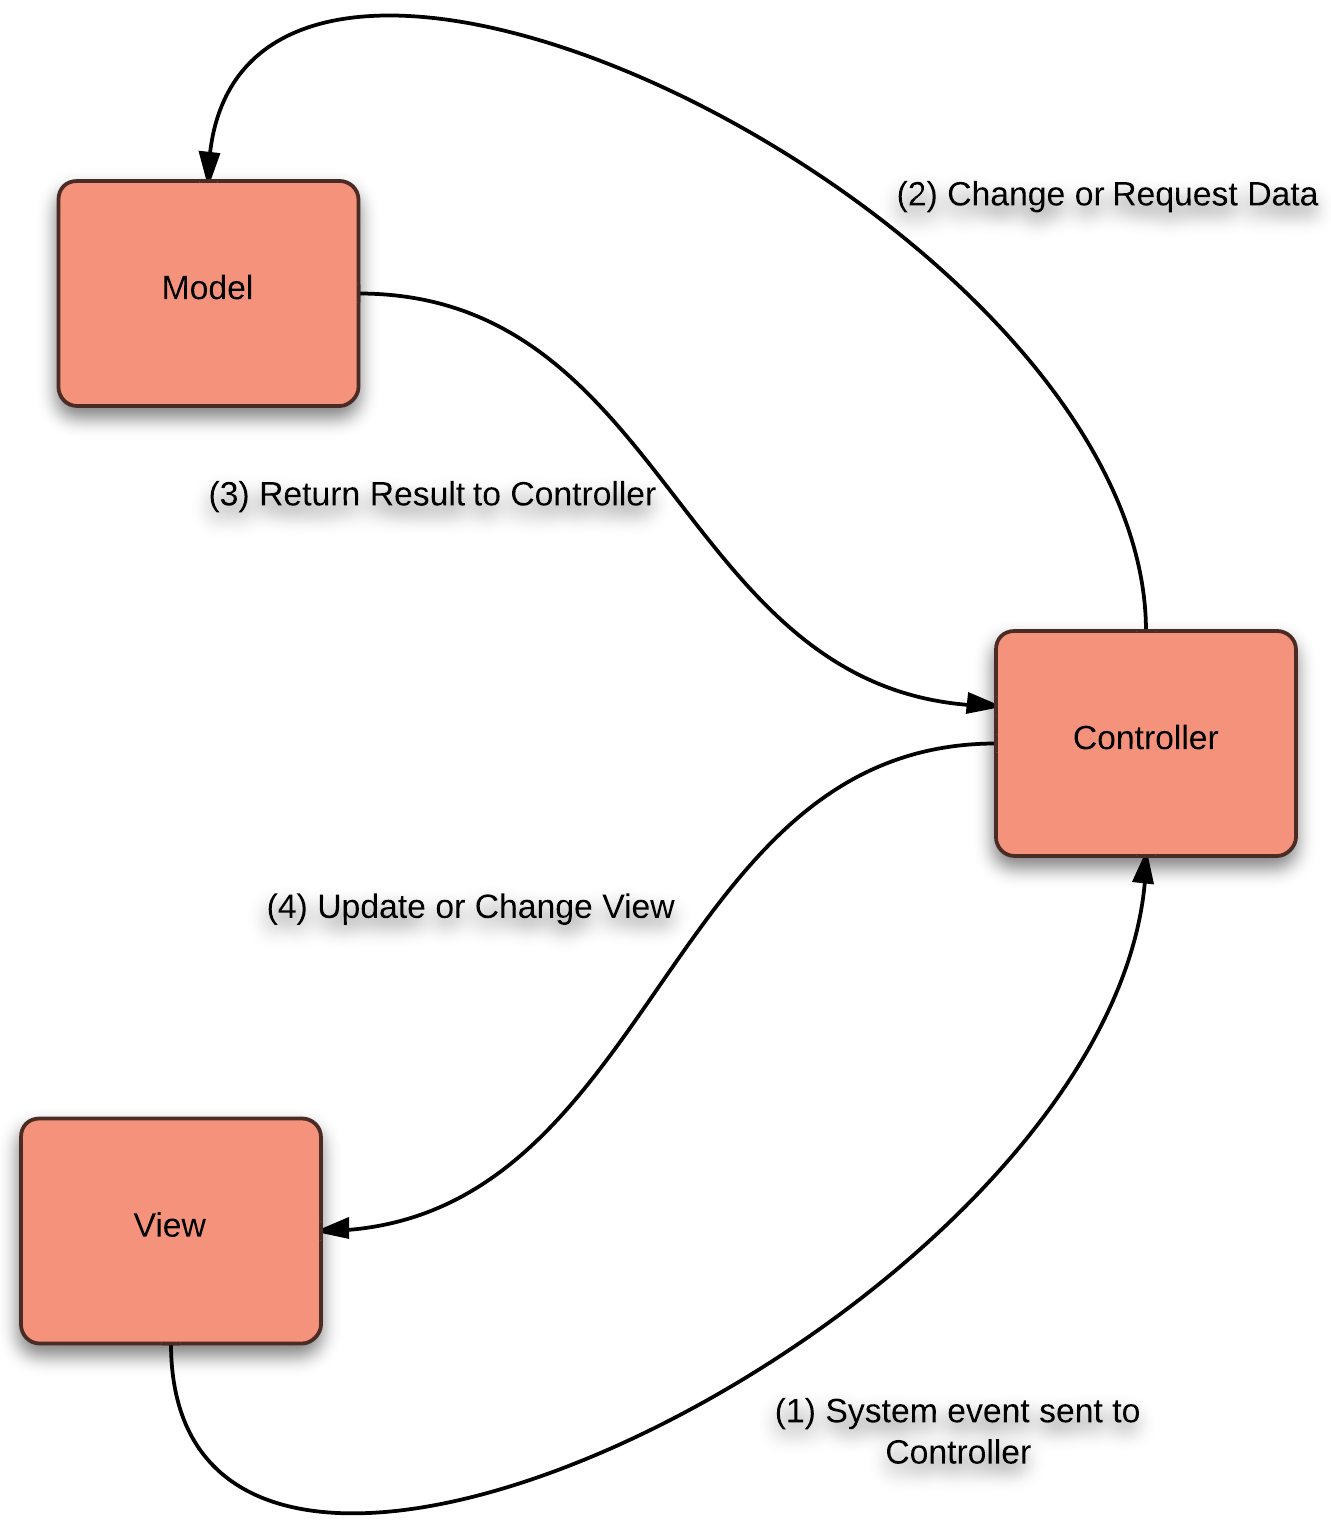
\includegraphics[width=9cm]{mvcclassic.png}
\end{center}
\caption{Classic MVC}
\label{fig:mvcclassic}
\end{figure}



Spring MVC has a \textit{DispatcherServlet}. This is defined within the \textit{web.xml} file, shown in Figure ~\ref{fig:webxml}. This file is located in the WEB-INF folder. Its purpose is to load the application context from a servlet file, defined within this application as \textit{member-servlet.xml}. An Application Context is an interface within the framework. This interface provides the configuration for the application. 

Spring MVC provides a clear separation of roles. Each role, such as a View, Controller, Mapper, Validator, Model and View Resolver, can be encapsulated within a relevant object. It is a request driven framework designed around the \textit{DispatcherServlet}. 

\begin{figure}[H]
\begin{center}
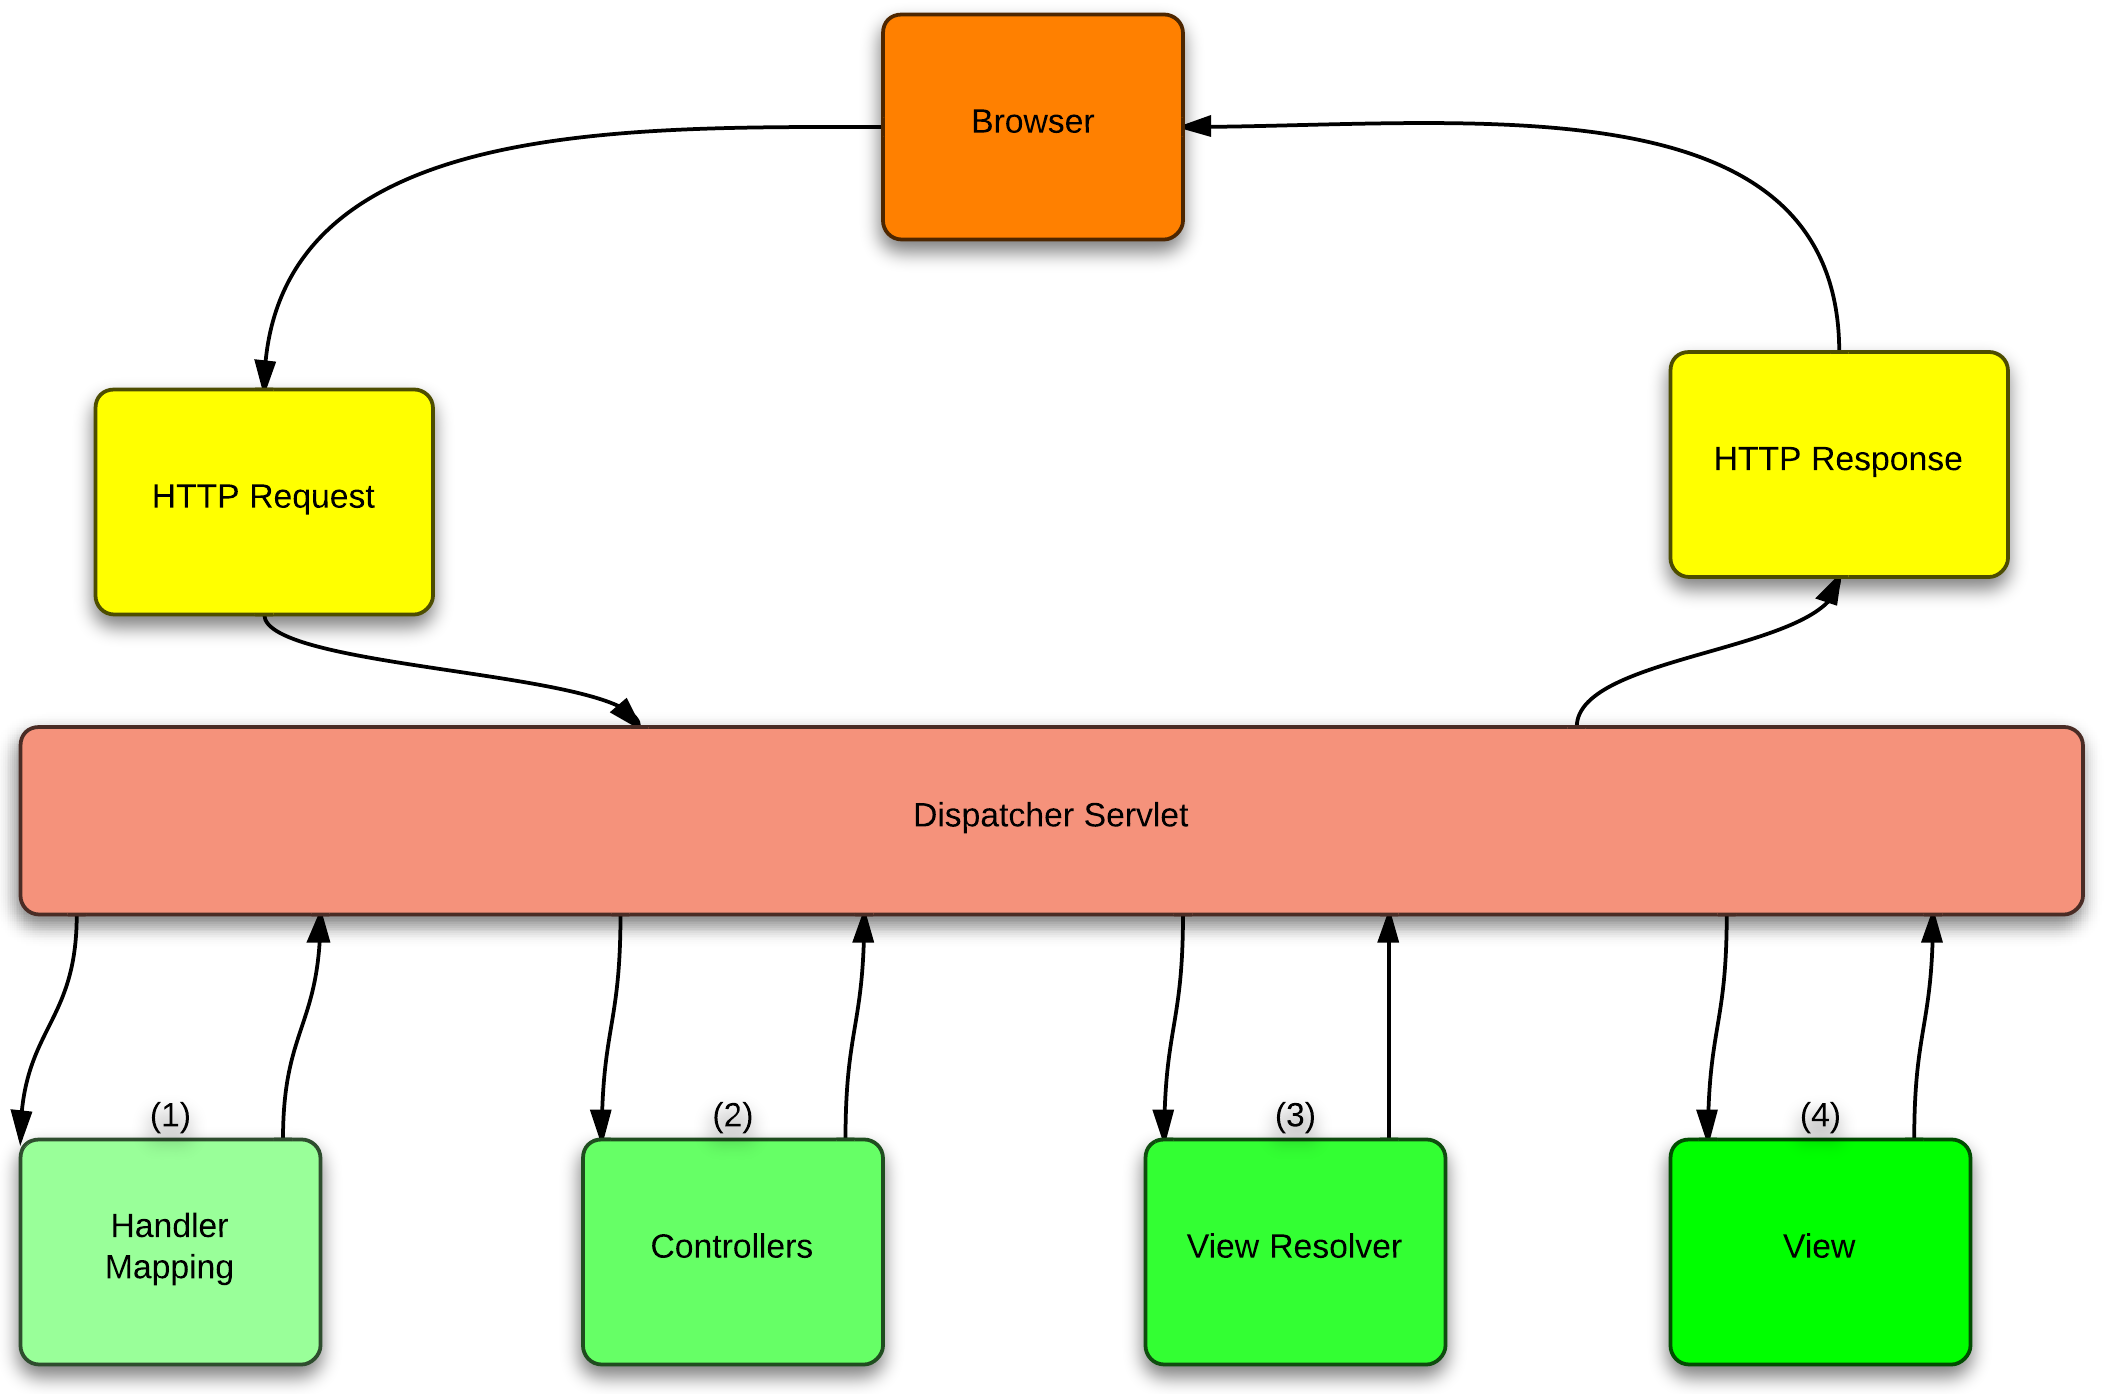
\includegraphics[width=14cm]{dispatchservlet.png}
\end{center}
\caption{DispatcherServlet}
\label{fig:dispatcherflow}
\end{figure}

The \textit{DispatcherServlet} is responsible for handling HTTP requests from the browser. Once it receives these requests, it consults the HandlerMapper, which calls the appropriate Controller. A HandlerMapper takes a value, such as "/admin", and checks which controller handles this mapping. The Controller will take this request, and call the appropriate method, or methods, and interact with the Service layer of the application, if necessary. The View name is then returned to the \textit{DispatcherServlet}, which in turn passes the value to the ViewResolver. 

A ViewResolver provides a mapping between a \textit{view name} and the \textit{view}, that is to say, the web page requested. Once this view is finalised, the \textit{DispatcherServlet} passed any model created within the Controller to the View, which is then rendered by the browser. This process is shown in Figure ~\ref{fig:dispatcherflow}


\begin{lstlisting}
<web-app 
xmlns:xsi="http://www.w3.org/2001/XMLSchema-instance" 
xmlns="http://java.sun.com/xml/ns/javaee" 
xsi:schemaLocation="http://java.sun.com/xml/ns/javaee http://java.sun.com/xml/ns/javaee/web-app_2_5.xsd" 
version="2.5">
  <display-name>monaleen-tennis</display-name>
  <welcome-file-list>
    <welcome-file>index.jsp</welcome-file>
  </welcome-file-list>
  <servlet>
    <description></description>
    <display-name>members</display-name>
    <servlet-name>members</servlet-name>
    <servlet-class>org.springframework.web.servlet.DispatcherServlet</servlet-class>
    <load-on-startup>1</load-on-startup>
  </servlet>
  <servlet-mapping>
    <servlet-name>members</servlet-name>
    <url-pattern>/</url-pattern>
  </servlet-mapping>
  <description>Database</description>
  <resource-ref>
    <description>DB Connection</description>
    <res-ref-name>jdbc/mtc</res-ref-name>
    <res-type>javax.sql.DataSource</res-type>
    <res-auth>Container</res-auth>
  </resource-ref>
  <context-param>
    <param-name>contextConfigLocation</param-name>
    <param-value>
	classpath:beans/dao-context.xml
	classpath:beans/service-context.xml
	classpath:beans/security-context.xml
	</param-value>
  </context-param>
</web-app>
\end{lstlisting}
\begin{figure}[H]
\caption{Spring DispatcherServlet Configuration}
\label{fig:webxml}
\end{figure}

Figure ~\ref{fig:webxml} is the configuration file needed for the \textit{DispatcherServlet}. The file has a number of responsibilities within the application.

\begin{table}[H]
\caption{DispatcherServlet Code}
\begin{itemize}
\item Define DispatcherServlet
\begin{itemize}
\item Line 9: This defines what class the DispatcherServlet implements.
\end{itemize}
\item Define ApplicationContext
\begin{itemize}
\item Line 17-19: This specifies the file that defines the application context of the application
\end{itemize}
\item Define DataSource
\begin{itemize}
\item Lines 22-27: This defines the reference to the database, and the DataSource class
\end{itemize}
\item Define Context Config Location
\begin{itemize}
\item Lines 28-35: This defines the files that contain the configuration for the DAO, Service and Security context files.
\end{itemize}
\end{itemize}
\label{fig:webxmlExplain}
\end{table}

The \textit{Controller}, within the Spring MVC framework, is designed for preparing a model with data, and selecting a view which will represent that data. This is done through the use of a \textit{RequestMapping} annotation, which is discussed in further detail in Section~\ref{sec:impl} of this report.

The default \textit{ViewResolver} within the Spring MVC is the InteralResourceViewResolver, depicted in Figure ~\ref{fig:defaultViewRes}. This is defined with the \textit{members-servlet.xml} file in the application, which is the structure of the \textit{DispatcherServlet}. This class takes the value that is returned by a Controller, and passes a View to the DispatcherServlet. The browser can then render this view. It is important that any views, such as JSP files within the scope of this application, are stored within the \textit{WEB-INF} folder. This is to ensure that the files are treated as an internal resource, and as such, are only accessible by the servlet, or the Controller classes within the application.

\begin{lstlisting}
<bean id="jspViewResolver"
	class="org.springframework.web.servlet.view.InternalResourceViewResolver">
	<property name="prefix" value="/WEB-INF/jsps/"></property>
	<property name="suffix" value=".jsp"></property>
</bean>
\end{lstlisting}
\begin{figure}[H]
\caption{Default ViewResolver Configuration}
\label{fig:defaultViewRes}
\end{figure}

This \textit{ViewResolver} was not used within this application. Instead, Apache Tiles provides its own \textit{ViewResolver}. This is due to the changes in how JSP pages are constructed and displayed by Apache Tiles, as discussed in the next section.

\subsection{View Resolver}

The framework that provided the \textit{ViewResolver} for this application was Apache Tiles. This framework allows for the composition of a template for a JSP page. Apache Tiles allows the application developer to define page fragments, which are assembled into one page at run time, based on a template. This allows the application to reduce duplication of common page elements, such as headers, footers, link bar and advertising.  The defined templates allow for a consistent look and feel across the application, and a change in one place, such as modifying a link in a header, will change across all Views within the application.

In order to use the Apache Tiles \textit{ViewResolver}, it must be defined within the \textit{DispatcherServlet} XML file, see Figure ~\ref{fig:tilesViewRes}, in lieu of the default ViewResolver. This ViewResolver is part of the Spring Framework, and allows for interoperability between both the Spring and Apache Tiles frameworks. The reason that \textit{TilesViewResolver} is used instead of \textit{SimpleTilesListener} is for the support of JSTL within the JSP pages, as discussed within the Implementation.

\begin{lstlisting}
<bean id="tilesViewResolver"
	class="org.springframework.web.servlet.view.tiles2.TilesViewResolver">
</bean>
\end{lstlisting}
\begin{figure}[H]
\caption{Default ViewResolver Configuration}
\label{fig:tilesViewRes}
\end{figure}

\subsection{Application Server}

The application server, or web server, used for this project was Tomcat 7.  Tomcat is an open source project by Apache, which is a software implementation of Java Servlet and JavaServer Pages technologies. This application provides an environment in which Java code can run. Tomcat has a servlet-container called Catalina. A servlet container is the part of the web server that interacts with the servlets created by the application. It manages the life-cycle of the servlets, and is responsible for specifying the run time environment for the components within the application, and delivering this content. This includes security, transaction management, deployment and other services. 

\subsection{Project Management Tool}

The project management tool used for this project was Maven. Maven was used within the scope of this project to manage the dependencies required by the web application. Maven came pre-installed and configured within the Spring Tool Suite IDE. Dependency Management can be handled one of two ways. Dependencies can be added using the GUI interface provided by an IDE, in this case, Spring Tool Suite. This GUI links to the repository located at http://mvnrepository.com/, and the user searches for the required files. Otherwise, the \textit{pom.xml} file may be edited to define dependencies manually. Below is an example of the Apache Tiles v3.0.3 dependency.

\begin{figure}[H]
\begin{lstlisting}
<dependency>
	<groupId>org.apache.tiles</groupId>
	<artifactId>tiles-core</artifactId>
	<version>3.0.3</version>
</dependency>
\end{lstlisting}
\caption{Dependency XML Structure for Maven}
\end{figure}

Maven also provided the archetype, or structure, for the application. It defined the folder structure for both the production and tests environments. It also sets up JUnit within the project to support unit testing throughout the development phase.

\subsection{Database Model}

The database framework used within this project was the open source framework, Hibernate. Hibernate is an Object/Relational Mapping [ORM] solution, and is concerned with relational databases, and more importantly for programmers, objects. Programmers generally "prefer to work with persistent data held (for the moment, anyway) in program objects, rather than use SQL directly for data access" \parencite{bauer2005hibernate}. 

Hibernate implements an Entity Data Model, and "sits between the object world of applications and the underlying database(s)" \parencite{bauer2005hibernate}. Hibernate is derived from the Java Persistence API (JPA) and can be used in any environment that supports JPA, such as Java EE, Java SE and Enterprise applications.

It manages objects that need to be persisted, known as Entity Classes [EC], using annotations, which are detailed in subsequent sections. Each EC has a unique identifier "whose value is not important to the application apart from its use as an identifier" \parencite{bauer2005hibernate}. 

A rudimentary examination of Hibernate with Java Database Connectivity [JDBC] will be completed with regards towards the CRUD operations of each ORM database. This is examined within the Evaluation section of this report.

\subsection{Integrated Development Environment}

The IDE used for this project was Spring Tool Suite [STS], a modified version of the open source IDE, Eclipse. The advantages of using STS over Eclipse are the pre configured services within the application. Tomcat, Maven, egit, and the core Spring dependencies themselves come pre-packaged within the application. Java EE and web application support are also present. One clear advantage of using STS over Eclipse is that if a organisation were using Eclipse as as IDE, they could be running a variety of different versions of application servers or plug ins. A pre-packaged solution like STS reduces the risks of bugs being introduced, or not being able to reproduce bugs, on different development environments.

\subsection{Source Control}

Source Control is the management of changes to the source code of an application. In this day and age, it is not unusual for a program to be worked on by a number of different persons. In fact, it is more likely to be a globally dispersed team of programmers, so management of changes to the code base is very important. Essentially, it is a system that "provides facilities for storing, updating and retrieving all versions of modules, for controlling updating privileges, for identifying load modules by version number, and for recording who made each software change" \parencite{rochkind1975source}.

The source control system used within this project was GitHub, a free open source solution located at \href{http://www.github.com}{www.github.com}. It provides integration with STS through the use of the \textit{egit} plugin, as well as GUI and Shell user interfaces for a variety of user systems. It was also used to manage the different versions of the report you are reading now. Within the scope of GitHub, each project is called a repository.

GitHub also provides graphs and statistics about each repository, such as which days are the busiest for commits as shown in Figure ~\ref{fig:git}, the growth of the code base over time and many more.

\begin{figure}[H]
\begin{center}
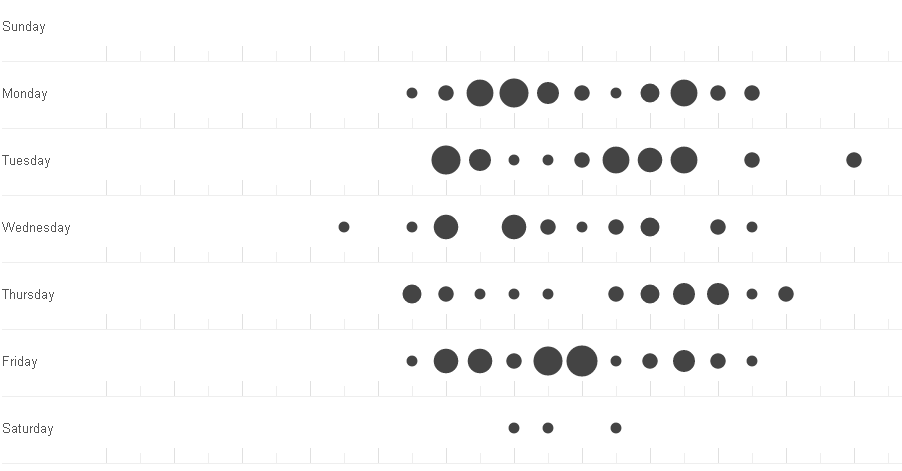
\includegraphics[width=15cm]{git.png}
\end{center}
\caption{GitHub Visualisation of Commits/Day}
\label{fig:git}
\end{figure}

\subsection{Logging}

Logging was used within the application to check both the flow of the application, as well as to pin point where certain lines of code were being called. The logging implementation used was log4j, an open source logging solution created by Apache. Log4j is designed with the possibility of enabling or disabling logging at run time. This is important in an application may have thousands of logging instances within it. This would be difficult to remove from production code, and would increase the risk of introducing bugs were it to be attempted. 

Logging can also be used to analyse usability and a "log will contain statistics about the frequency with which each user has used each feature in the program and the frequency with which various events of interest (such as error messages) have occurred." \parencite{holzinger2005usability}

\section{Usability Studies}

The important criteria that govern usability were looked at within this project. In doing this, two other websites were examined: the current website for the club, and a site that was recommended to me by a club member, Tralee Tennis club. For this task, usability studies by Jakob Nielson were examined. 

\subsection{Case Study: Monaleen GAA Tennis Club}

The first site examined was the existing site for the club. This site is located at \newline\textit{http://www.monaleengaatennisclub.com/}. The current site is a basic HTML site with a CSS stylesheet, that occasionally uses a PHP script to facilitate users to register for tournaments. It uses a basic architecture stack consisting of these HTML pages coupled with an Apache HTTP Server. The reasons for this choice that the club just needed a presence on the internet, there was no need for much functionality at the time, and simplicity.

This architectural choice places a number of constraints on the potential growth of the site however. The definition of roles within the system is not possible. An example would be that committee members cannot add news stories themselves, but must contain the web-master to perform this action on their behalf. There is also no scope to add secure features to the site, such as a members only feature. Any introduction of these features would require a considerable overhaul of the existing architecture.

The only NFR looked at during the development of the site was availability, which is fulfilled by the choice of architecture and lightweight implementation. 

(usability stuff will go here, leading onto sites that were admired by the club (ie Tralee))

\subsection{Case Study: Tralee Tennis Club}
\chapter{Requirements}
\label{requirements}

\section{Introduction}

Requirements Elicitation is an important step in the development of a software application. There are a number of techniques possible, such as "interviewing, protocol analysis, repertory grid, work groups" \parencite{davis2006effectiveness}. Structured interviews "appear to be one of the most effective elicitation techniques in a wide range of domains and situations" \parencite{davis2006effectiveness}. 

In eliciting possible requirements for the site, there was a discussion with three club members with varying backgrounds and experience within the club.

\begin{table}[H]
\caption{Stakeholders for Requirements Elicitation}
\begin{center}
    \begin{tabular}{ | l | l | l | l | l| p{5cm} |}
    \hline
    Name & Age Bracket & Club Role & Club Membership & Work Background \\ \hline
	S1 & 35 - 45& Committee Member & 5 years & Senior Software Engineer \\ \hline
	S2 & 18 - 25 & New Member & 1 year & Graduate Software Engineer \\ \hline
	S3 & 55+ & Senior Member & 10+ years & Retired Public Servant \\ \hline
    \end{tabular}
\end{center}
\label{fig:userelicit}
\end{table}

\section{Methods for Requirements Elicitation}

\subsection{Storyboarding}

At an early stage of the application, rough storyboards were prepared for the FYP presentation. These storyboards were used to demonstrate how a page, such as the timetable shown in Figure~\ref{fig:timetableSB}, would be displayed by the application.

\begin{figure}[H]
\begin{center}
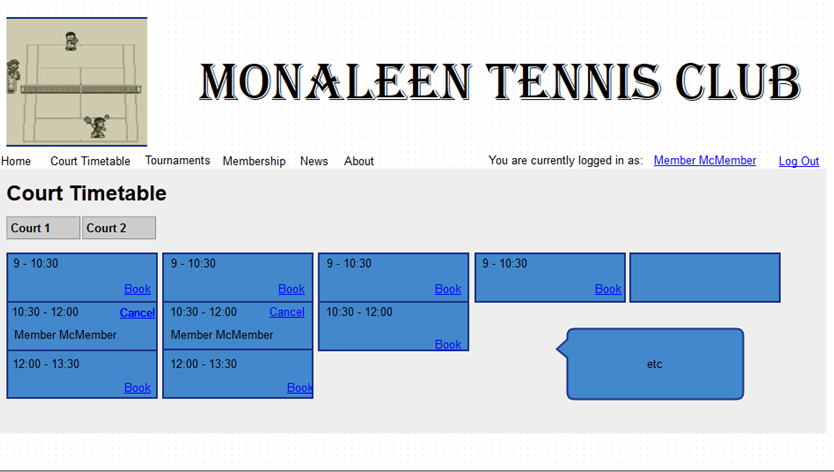
\includegraphics[width=14cm]{storyboard.png}
\end{center}
\caption{Timetable Storyboard, October 2013}
\label{fig:timetableSB}
\end{figure}

The storyboarding visualised aspects of the site, and gave a rough idea of functionality that would be needed within the application. 

\subsection{Interviews}

In order to elicit requirements, a number of interviews were held with stakeholders. These questions are listed in~\ref{sec:regquestions},~\nameref{sec:regquestions}.

During the elicition process a number of areas were highlight as desired features.

\begin{enumerate}
\item Online Timetable
\begin{itemize}
\item Allow members to view courts and make/view bookings
\end{itemize}
\item Tournaments
\begin{itemize}
\item Allow user to register for a tournament, and view tournaments ongoing.
\end{itemize}
\item Contact Members
\begin{itemize}
\item Easy way to contact all members
\end{itemize}
\item Member Directory
\begin{itemize}
\item A list of all members, contact details, roles
\end{itemize}
\item News Section
\begin{itemize}
\item Create new items to display for members
\end{itemize}
\item Members Area
\begin{itemize}
\item A secure area that only members could access
\end{itemize}
\item Member Application
\begin{itemize}
\item Automated registration, replace old paper form
\end{itemize}
\item Club Map
\begin{itemize}
\item Directions to the club for new members and non-local visitors
\end{itemize}
\item Contact Details
\begin{itemize}
\item Information on how to contact within the club for specific needs
\end{itemize}
\item Statistics
\begin{itemize}
\item Such as games played, Win/Loss ratio
\end{itemize}
\end{enumerate}
\begin{table}[H]
\label{fig:requirementsFeatures}
\caption{Requested Features}
\end{table}
Table ~\ref{fig:reqbreakdown} refers to each numbered requirement, and whether it was brought up by a stakeholder during the elicitation process.
\begin{table}[H]
\caption{Requested Feature Breakdown}
\begin{center}
    \begin{tabular}{ | l | l | l | l| l| l| l| l| l|l| p{.22cm} |}
    \hline
     \textit{Name}& 1& 2 & 3 & 4 & 5 & 6 & 7 & 8 & 9 & 10\\ \hline
	 S1 & N & Y & Y & Y & Y & Y & Y & Y & Y & N\\ \hline
	 S2 & Y & Y & Y & N & N & N & N & N & N & Y\\ \hline
	 S3 & Y & N & N & N & N & N & Y & Y & N & N\\ \hline
  Total & 2 & 2 & 2 & 1 & 1 & 1 & 2 & 2 & 1 & 1\\ \hline
    \end{tabular}
\end{center}
\label{fig:reqbreakdown}
\end{table}

This features were broken down into four categories: \textit{Timetable}, \textit{Tournaments}, \textit{Members}, and \textit{News}.

\section{Application}

\section{Functional Requirements}



\subsection{Timetable} 

The timetable is the core aspect of the application, and one that would be most likely to be used by all members, not just those involved competitively. While the regular member would only be concerned with the booking of slots, there are a number of requirements defined for use by the administrator in order to configure a relevant timetable not the club. The timetable needs to be flexible to allow the administrator full control at all stages.

\begin{enumerate}
\item Flexible 
\item Edit individual slots
\item Define a template for a timetable
\item Reset timetable
\item Define look ahead for timetable (how many weeks in advance a user can see)
\item Delete timetable
\item Enable and disable timetable
\item Timetable analysis (No slots free, booked etc)
\end{enumerate}

\subsection{Tournament}

\subsection{News}

\subsection{Members}

\section{Use Cases}

\begin{usecase}
\addtitle{Use Case 1}{View All Members} 
\addfield{Scope:}{System-wide}
\addfield{Level:}{User can view a list of all registered, and approved, members of the club}
\addfield{Primary Actor:}{All Registered and Authenticated Users}
\additemizedfield{Stakeholders and Interests:}{
	\item All Users: contact information for club members
}

\addfield{Preconditions:}{User is registered and approved}
\addfield{Postconditions:}{User must be authenticated by the framework}
\addscenario{Main Success Scenario:}{
	\item User logs in
	\item User clicks on View Members
	\item System displays member information
}
\addscenario{Extensions:}{
	\item[1.a] Invalid login data:
		\begin{enumerate}
		\item[1.] System shows failure message
		\item[2.] User returns to step 1
		\end{enumerate}
	\item[1.a] User not approved:
		\begin{enumerate}
		\item[1.] System shows failure message
		\item[2.] Admin is emailed about attempted access by unapproved member
		\end{enumerate}
}
\addfield{Frequency of Occurrence:}{High}
\end{usecase}

\section{Non Functional Requirements}

\subsection{Security}

Since user details would be stored in the application, security of this data was highlighted as a concern. While no payment information would be held by the application, there would be names, addresses and phones numbers held within the application. The security of this information would need to be ensured.

\subsection{Extensibility}

Extensibility of the application was discussed with particular attention of the ability of the application to deal with changed to the club structure. Currently, the club has two courts in which users can book time for games. It is likely that the club will be expanding in the near future. This will result in the creation of four next courts in the near future. The application should be able to scale with this possibility without issue.

Tournaments were also mentioned as an area where future requirements may stem from. Currently, the club operates three kinds of tournaments: Singles, Doubles and Mixed Doubles. These are broken down into Ladder style tournaments and Bracket style tournaments. The club regularly holds tournaments with other national tennis clubs. The ability to create tournaments that suit these events could be necessary.

\subsection{Usability}

The age of the club members range from 8 to 80, so ease of use of any software solution is important. If a system is going to replace the existing system that all can use, a similar level of usability is required. The most common function used by members is the reservation of time slot in one of the courts. A software alternative needs to be intuitive for all members.

\subsection{Performance}


\chapter{Design}
\label{design}

\section{Introduction}

The design of the application was crucial especially with the use of a number of software frameworks being used in its development. A number of design principles are encapsulated within these frameworks, and by using them, the programmer is implicitly using sound design practices within the application. 

\section{Framework Design}

Spring MVC and Hibernate incorporates a number of design patterns within its own classes. By using these frameworks, developers are guided towards best practice in terms of the application design


\begin{enumerate}
\item Singleton
\begin{itemize}
\item Beans defined within the Spring MVC framework and singletons by default. 
\end{itemize}
\item Factory
\begin{itemize}
\item The Factory pattern is used for loading Beans through the \textit{BeanFactory} class, and the \textit{Application Context}. 
\end{itemize}
\item Inversion of Control
\begin{itemize}
\item This pattern is central to the dependency injection facilities of the Spring framework, and is responsible for the instantiation of objects at run time, rather than compile time.
\end{itemize}
\newpage
\item Query Object
\begin{itemize}
\item This pattern is used by Hibernate with its Criterion object. This delegates the execution of a query to another object. 
\end{itemize}
\end{enumerate}

\label{sec:design}
\section{Controller-Service-DAO Design}

In order to achieve modularity across the application, the core of the application is separated into four key areas.

\begin{enumerate}
\item Entities
\begin{itemize}
\item A Java object that is persisted to a table in a relational database.
\end{itemize}
\item Controllers
\begin{itemize}
\item A controller will handled the user requests the application must deal with
\end{itemize}
\item Service
\begin{itemize}
\item The Service layer facilitates communication between the controller and the DAO layer.
\end{itemize}
\item Data Access Objects [DAO]
\begin{itemize}
\item This layer is responsible for persisting an entity or any changes to an entity.
\end{itemize}
\end{enumerate}
\begin{figure}[H]
\label{fig:appbreakdown}
\end{figure}

This structure follows a design principle called \textit{Separation of Concerns}. This separates an application into a number of component parts in order to minimise the effect that changes in one module have on other modules. In this application, any changes to the DAO layer will have no effect on the Controller layer for example. This is realised through this design principle, and the use of the Hibernate framework.

The flow between these objects is shown in Figure~\ref{fig:csdao}. An example flow would be the creation of a user objects. 

\begin{figure}[H]
\begin{center}
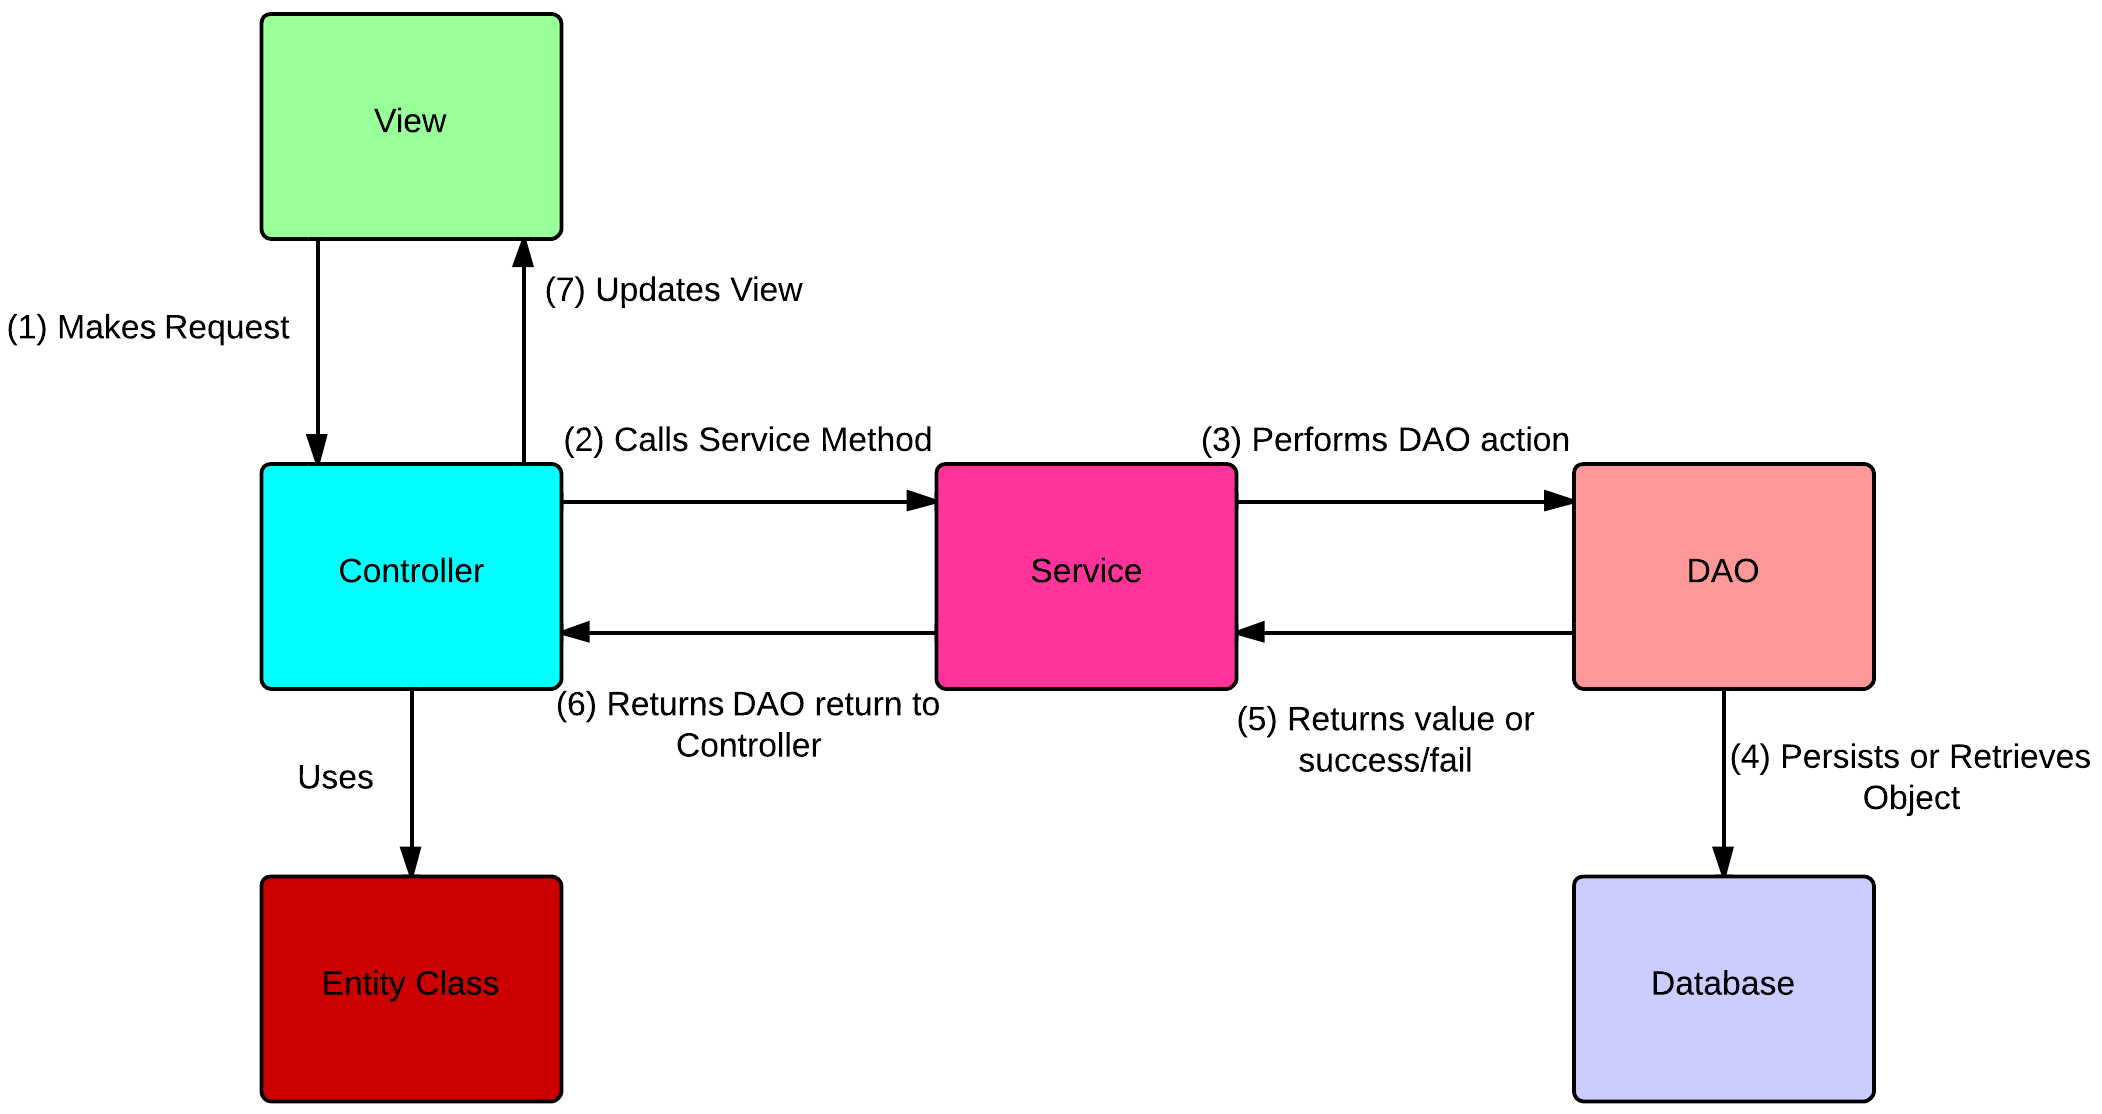
\includegraphics[width=14cm]{csdao.png}
\end{center}
\caption{Controller-Service-DAO Flow}
\label{fig:csdao}
\end{figure}

\subsection{User Roles}

The User class was designed with the existing application form of Monaleen Tennis Club as a foundation. 
Spring controls access within the application. Firstly, it uses an \textit{authority} hierarchy to separate different levels of users. For this web application, there were three main levels of authority, with one level containing three different branches.

\subsubsection{Roles}
\begin{itemize}
\item ROLE ADMIN
\begin{itemize}
\item This refers to the main administration group. The group retains full rights across the web application
\end{itemize}
\item ROLE COMMITTEE
\begin{itemize}
\item This refers to the committee, as defined by the club themselves. This group with have the ability to perform some administrator privileges, but only those directly related to club activities, not site activities.
\end{itemize}
\item ROLE MEMBER
\begin{itemize}
\item The default user state. This group can perform actions such as booking slots in a timetable, registering for a tournament, and will have access to parts of the site unavailable to non-registered users.
\end{itemize}
\item ROLE WARNING 
\begin{itemize}
\item A restriction placed upon a member. For example, a member who books time slots, but does not attend. In this application, it reduces the number of allowed bookings on a court per week from 3 to 2.
\end{itemize}
\item ROLE SUSPEND
\begin{itemize}
\item A further restriction placed upon a member. Number of bookings on a court per week reduced to 1.
\end{itemize}
\end{itemize}
\label{fig:secRoles}


\subsection{Database Design}

The database was designed using MySQL Workbench, and created using the same tool. The database Entity Relationship (ER) diagram is illustrated in Figure~\ref{fig:dbdesign}

\begin{figure}[H]
\begin{center}
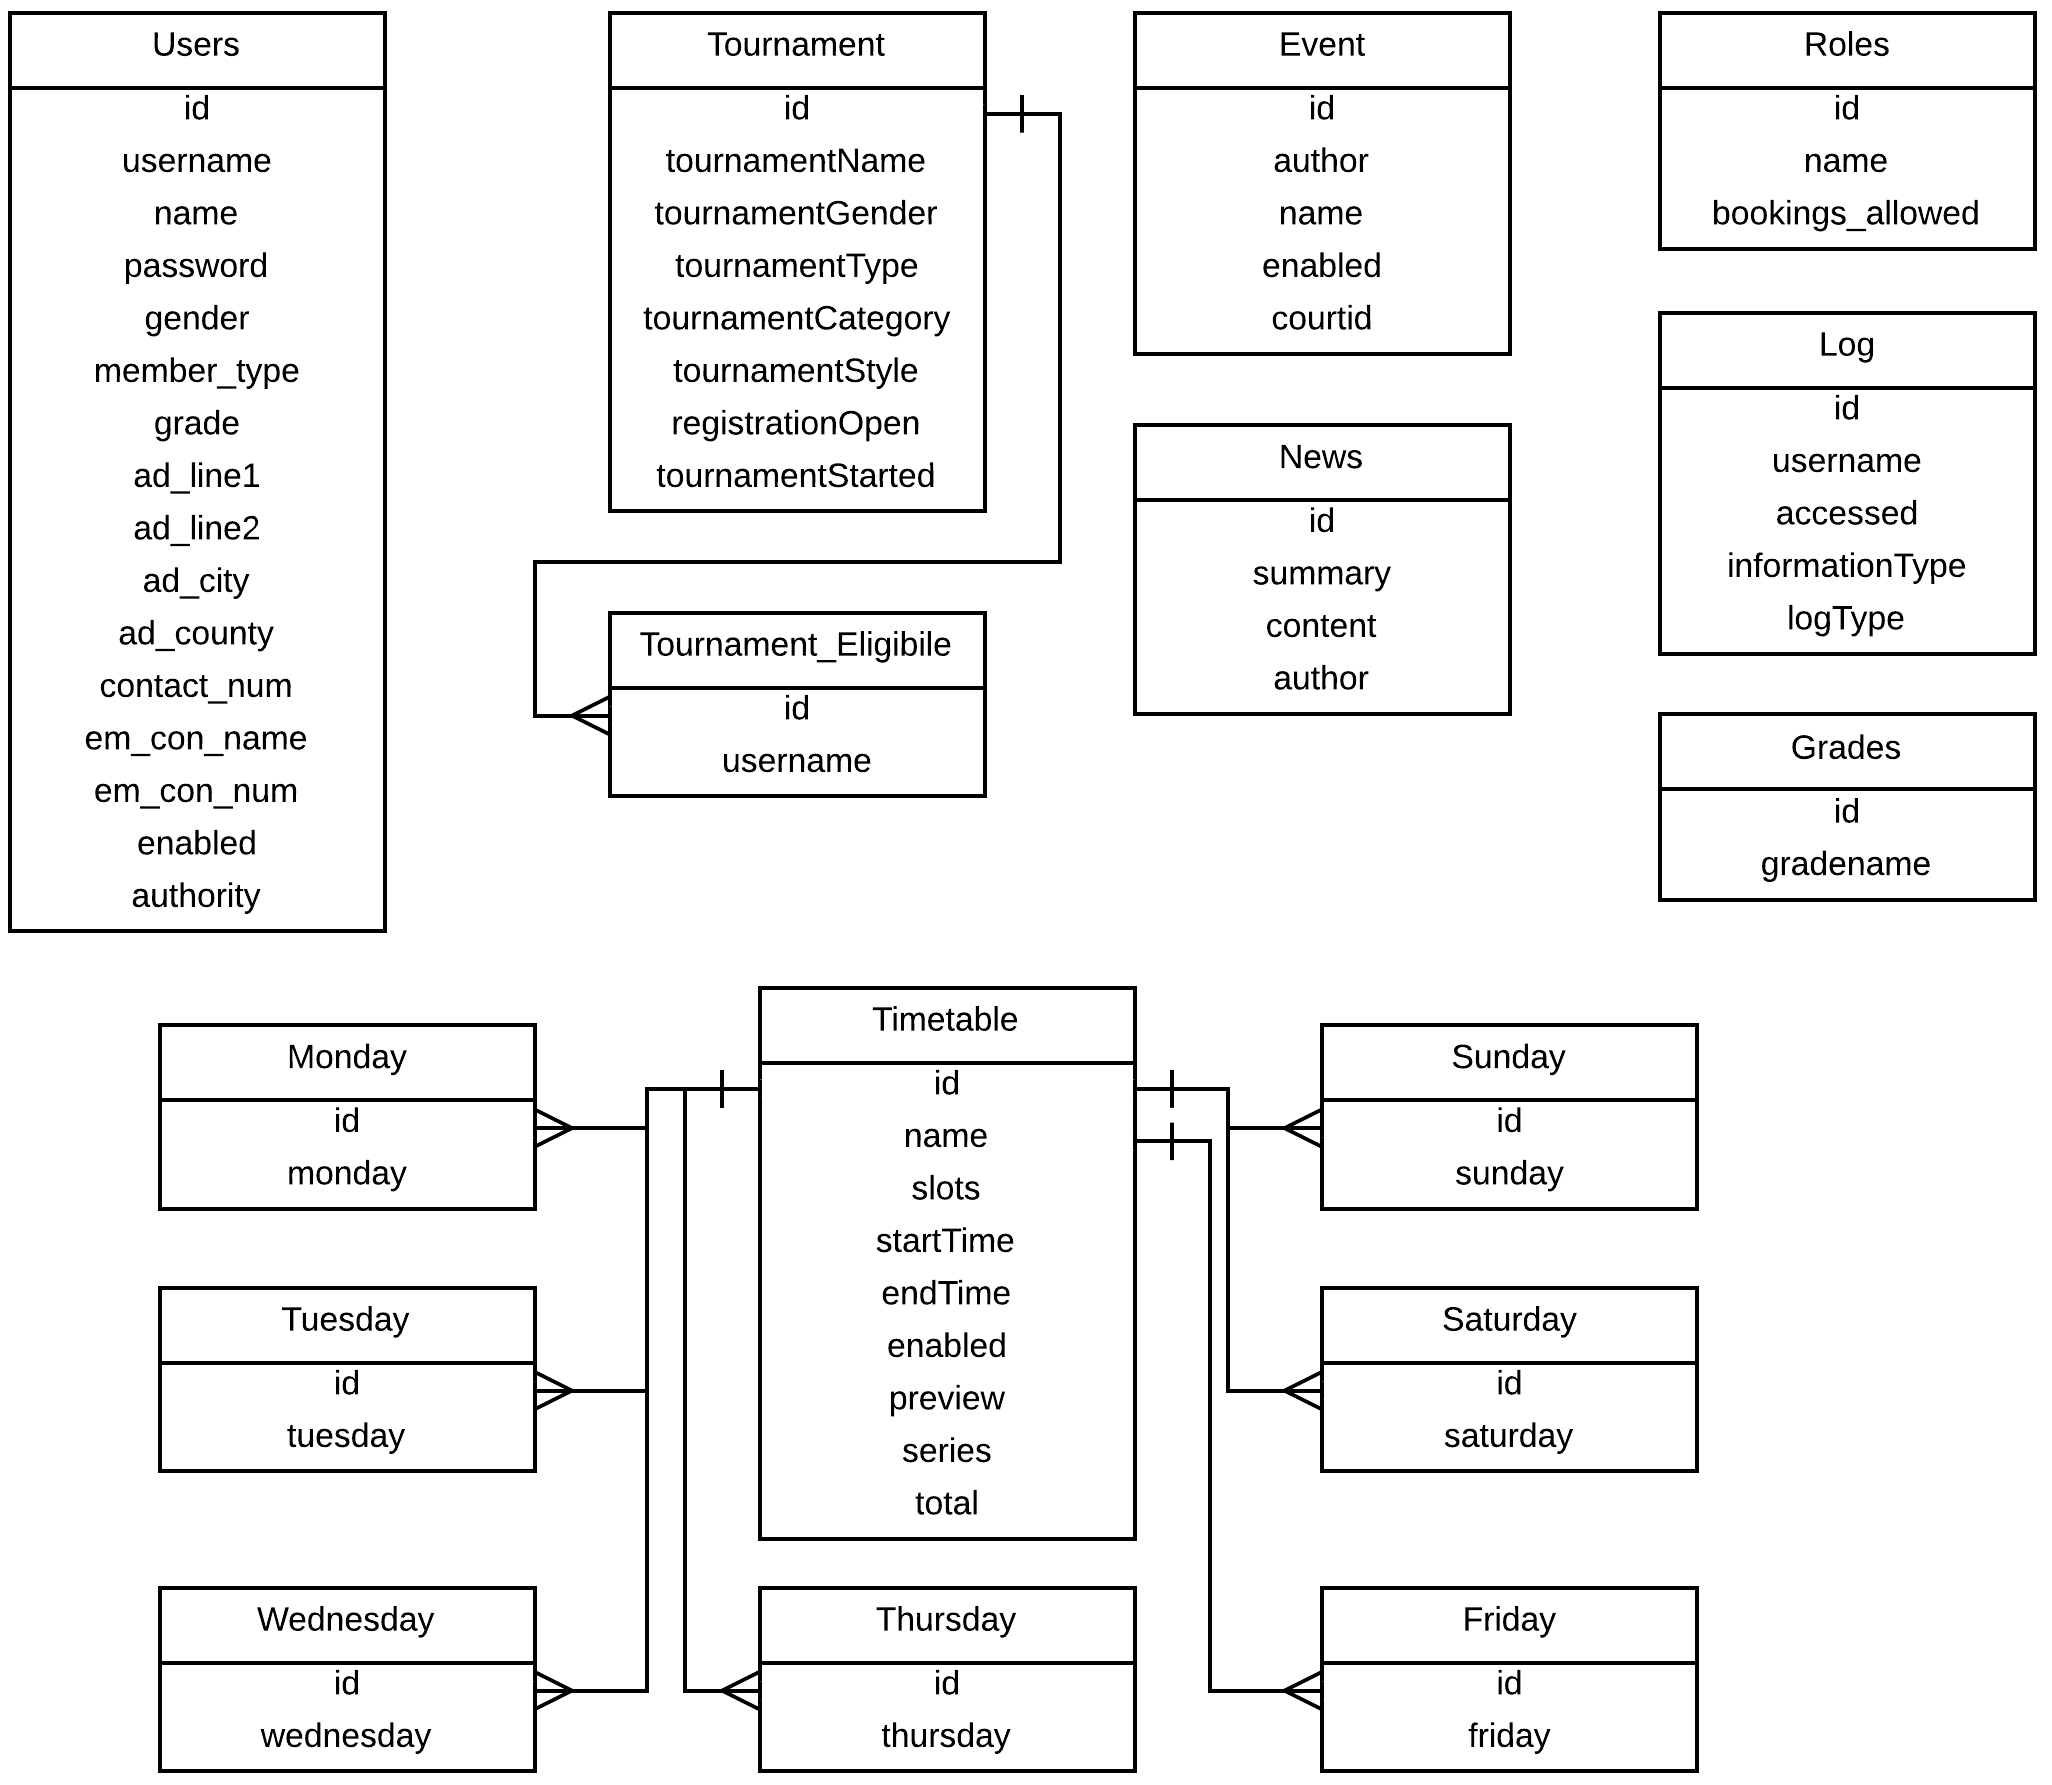
\includegraphics[width=14cm]{dbdesign.png}
\end{center}
\caption{Database Design}
\label{fig:dbdesign}
\end{figure}


\chapter{Implementation and Testing}
\label{impltesting}

\label{sec:impl}
\section{Introduction}

This chapters deals with the implementation of the application, with the focus on the application entities, and how they were configured.

\section{Application Entities}
\subsection{Users - Persistence}

The \textit{User} class represents every user account within the application. (Link to appendices showing class attributes). This section will focus on a regular user, how it is configured within the application in terms of bean definition and persistence. 

Firstly, as shown in line one of Figure ~\ref{fig:userDef}, the class needs to be configured as a \textit{Component} for the application. This ensures that the Spring framework considers the User class as one for auto-detection, through the use of class path scanning and annotations prevalent within this application. The framework instantiates this bean, or object, automatically, without the developer having to use the \textit{new} keyword.

\begin{figure}[H]
\begin{lstlisting}
@Component
@Entity
@Table(name="users")
public class User {
	@Id
	@GeneratedValue
	int id;
	
	@NotNull(groups={PersistenceValidationGroup.class, FormValidationGroup.class})
	@Pattern(regexp=".+\\@.+\\..+", message="This does not appear to be a valid email address", groups={PersistenceValidationGroup.class, FormValidationGroup.class})
	@Column(name="username")
	String username;
	
	@Size(min=5, max=45, message="Named must be between 5 and 45 characters",groups={PersistenceValidationGroup.class, FormValidationGroup.class})
	@Column(name="name")
	String name;
	
	@Column(name="password")
	@Size(min=5, max=15, message="Password must be between 5 and 15 characters", groups=FormValidationGroup.class)
	String password;
	
	@Column(name="gender")
	String gender;
	
	@Pattern(regexp="08[35679]([0-9]{7})", message="Number must be in the format 083, 085, 086, 087, 089 and 7 additional numbers eg 0851234567", groups={PersistenceValidationGroup.class, FormValidationGroup.class})
	@Column(name="contact_num")
	String contact_num;
	//Class truncated. Some repetitive attributes omitted
	//Getters and Setters below here.
\end{lstlisting}
\caption{User Class Definition and Configuration}
\label{fig:userDef}
\end{figure}

The \textit{Entity} and \textit{Table} annotations of lines 2 and 3 respectively belong to the javax.persistance package. These annotations are used by Hibernate in order to manage and persist the class. The \textit{@Table} annotation has a 'name' attribute that refers to the schema table the class maps to. There are two ways that an attribute can be assigned to a table column by Hibernate. Both methods are shown in Figure ~\ref{fig:userDef}. An annotation may be placed on the attribute in order to specify a column name. Line 12 in Figure ~\ref{fig:userDef} shows the username attribute being mapped to the username column within the User database schema. The other way of specifying where an attribute should be persisted is to ensure that the attribute name matches the column name within the table. This implicitly allows Hibernate to map a class, without having to explicitly define the mapping for the persistence framework.

The User class has a number of attribute constraints placed upon it. There are two types of constraints within this application: \textit{FormValidationGroup} and \textit{PersistenceValidationGroup}. These are interface classes with no attributes that serve as identifiers. As shown in lines 10, 14, 19 and 25 of Figure ~\ref{fig:userDef}, an attribute may be constrained by one or more groups. An annotation, from the javax.validation.constraints, is applied to the attribute. The annotations used within this application were as detailed in Table ~\ref{fig:classConstraints}.

\begin{table}[H]
\caption{Class Constraints}
\begin{center}
    \begin{tabular}{ | l | l | p{5cm} |}
    \hline
    Constraint Name & Description\\ \hline
	NotNull [Line 9] & Ensures the value within the attribute does not have a null value\\ \hline
	Pattern [Line 10] & Ensures the value within the attribute conforms to a regular expression\\ \hline
    @Size - Min [Line 14] & Ensures the value within the attribute has a minimum length\\ \hline
	@Size - Max [Line 14] & Ensures the value within the attribute has a maximum length\\ \hline

    \end{tabular}
\end{center}

\label{fig:classConstraints}
\end{table}

These validation package interfaces provide a \textit{groups} attribute, which is an array of objects. The \textit{FormValidationGroup} and \textit{PersistenceValidationGroup} are passed to this attribute. These groups allow attributes to have different constraints at different stages in the application. When using this attribute within the application, such as the creation of a user within a form, the Controller classes apply the validation to the user input and persisted data. The reason for having two groups of validation within this application is due to security. In every application, it is advisable to perform encryption on sensitive data, such as passwords. Within the scope of this application, user passwords were defined as being between 5 and 15 characters long, with no restriction to the content of the password. This application flow on taking in user input and persisting it is demonstrated below in Figure~\ref{fig:dbflow}.

\begin{figure}[H]
\begin{center}
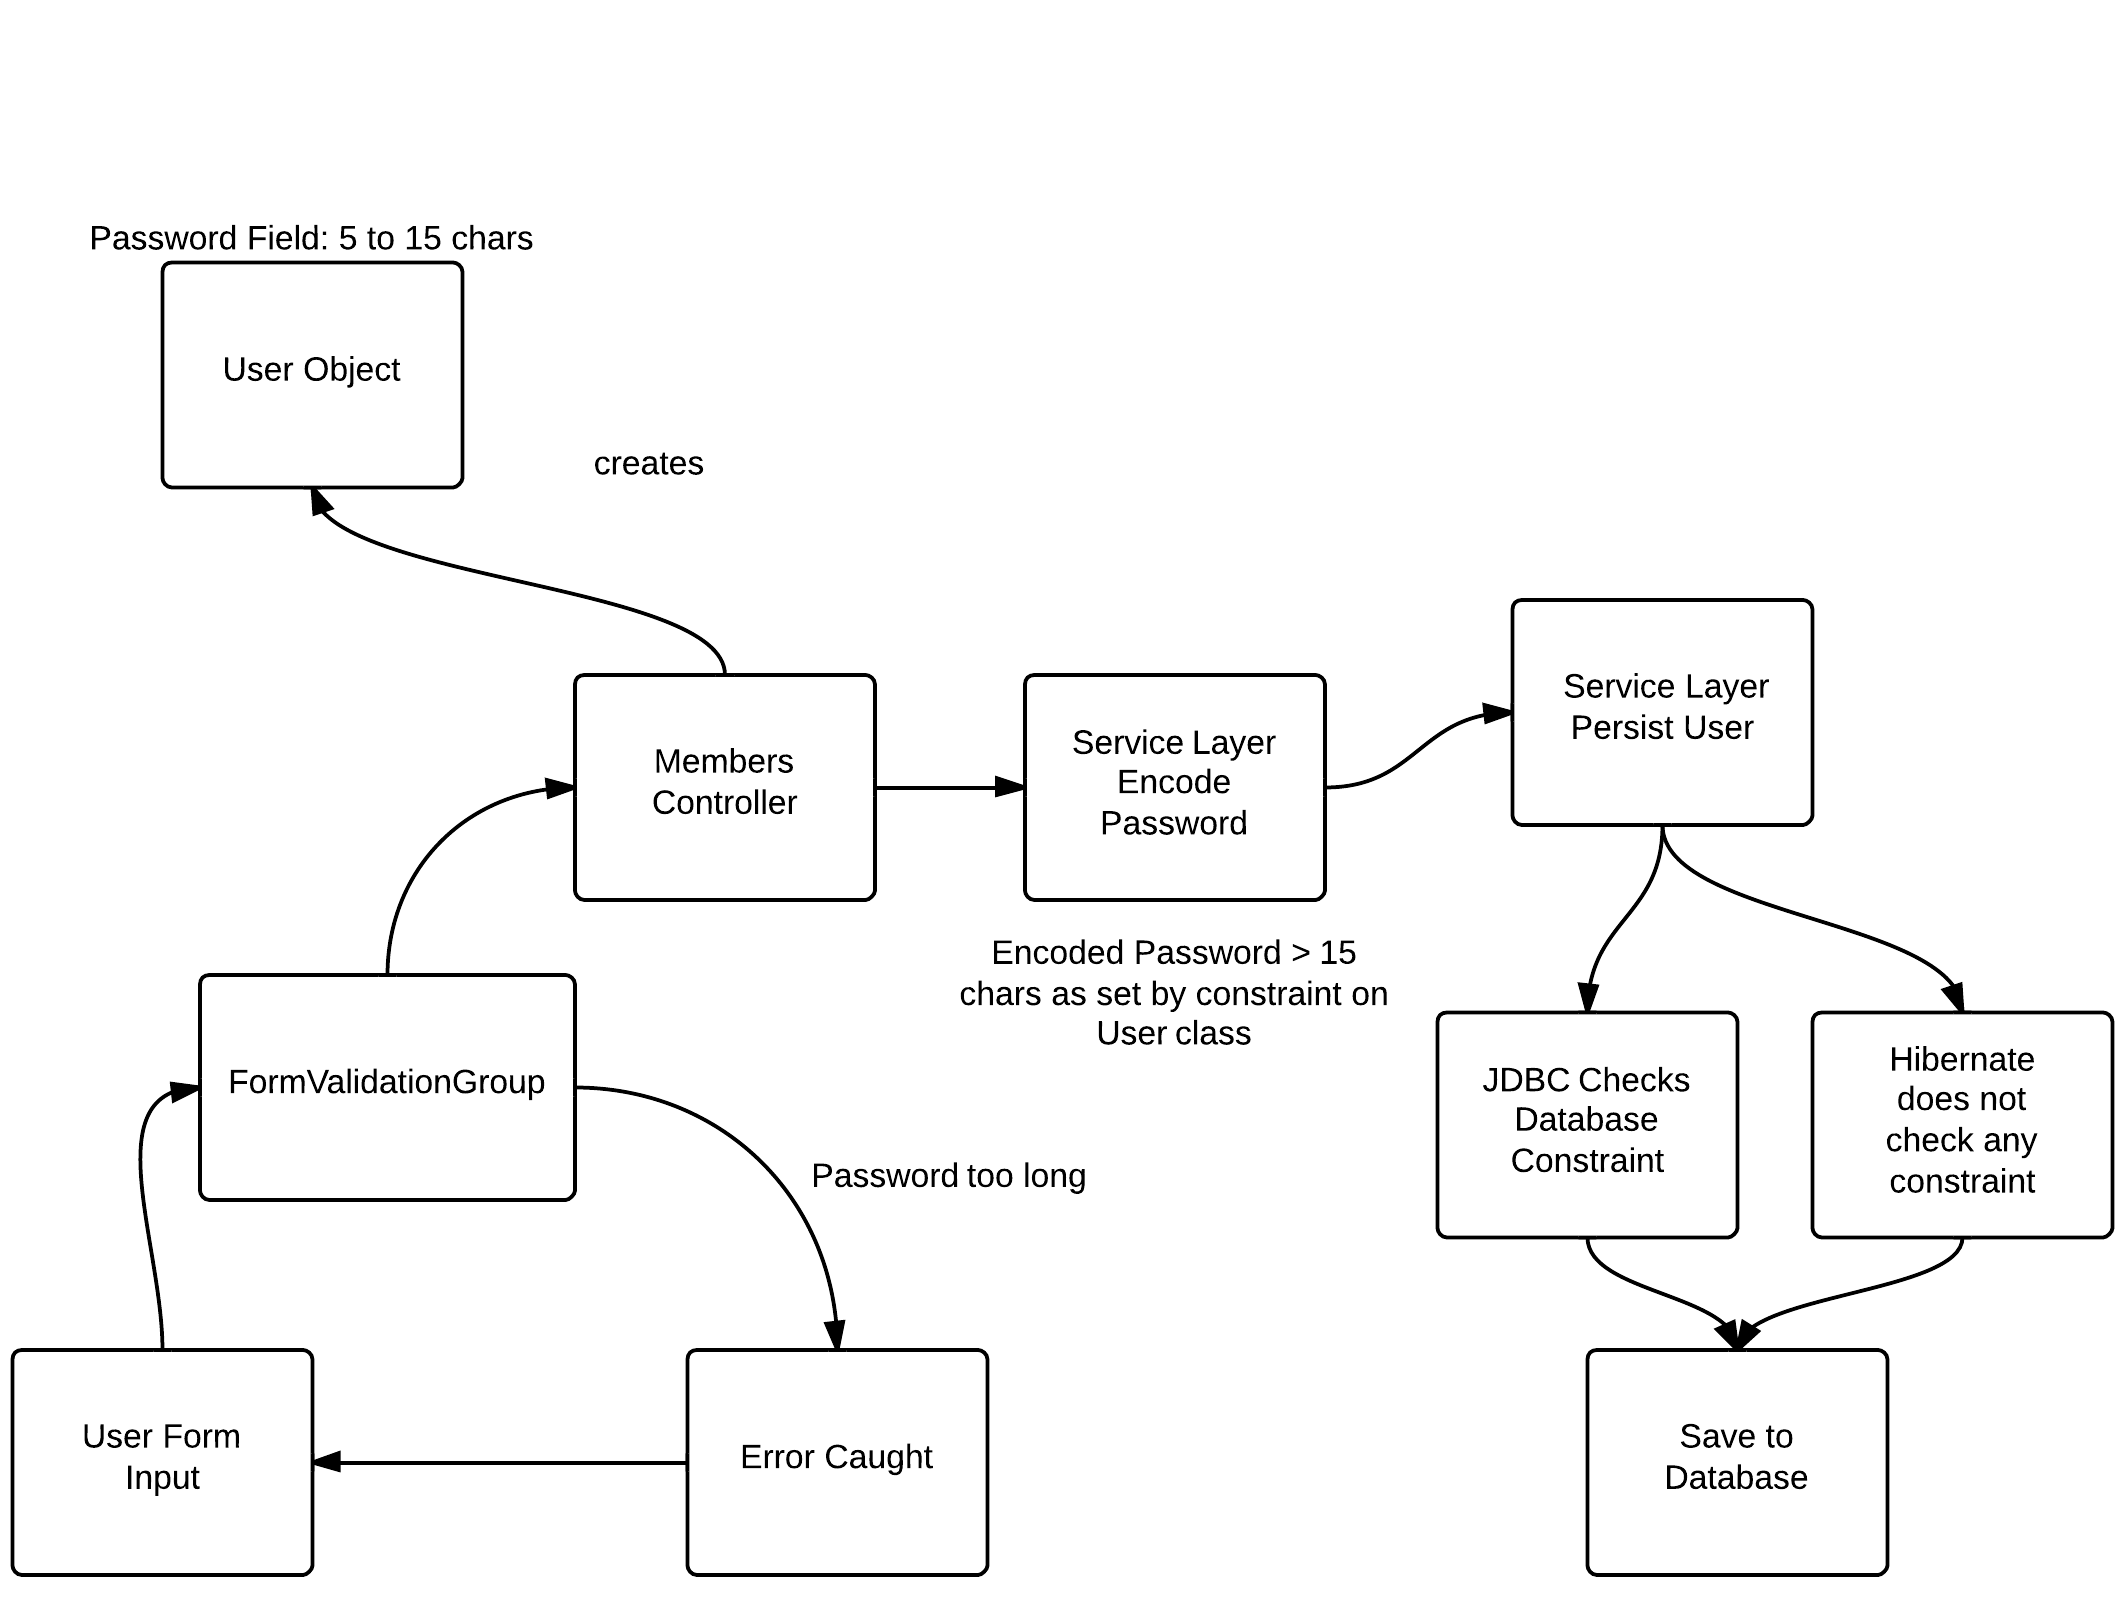
\includegraphics[width=14cm]{dbflow.png}
\end{center}
\caption{DispatcherServlet }
\label{fig:dispatcherflow}
\end{figure}

For example, a user password with 8 characters would pass form validation with no issues. When the PasswordEncoder bean is applied to the string prior to persistence, it will result in a value like \textit{'acb172137243c0b931321d7645dc31c2efb8346385ae0547d11b1d8de333215b'}, a value much longer than 15 characters. This will cause a failure with Hibernate persistence. This is because Hibernate works at a class level, and does take note of the constraints placed upon the class, while JDBC does not. The constraints that JDBC takes note of are those taken directly from the database itself. In this application, passing form validation is sufficient, as there are security annotations placed on the Service classes that manage data persistence. An example of how the controller handles validation is shown later in Figure ~\ref{fig:memberController}. 

Alongside class configuration, it is also necessary to configure Hibernate to scan the packages that contain entities, as detailed in Figure ~\ref{fig:hibernateConfig}. This is done through the creation of a sessionFactory bean, which uses the AnnotationSessionFactoryBean class. This bean is responsible for the creation of session instances within the application, though each application usually only has one session. It is an immutable object, and cannot be changed once it is created, so proper configuration of classes to facilitate object-relational mapping is important. The Session object created by the factory is responsible for creating the connection between the application and the database.

\begin{figure}[H]
\begin{lstlisting}
<bean id="sessionFactory"
class="org.springframework.orm.hibernate3.annotation.AnnotationSessionFactoryBean">
<property name="dataSource" ref="dataSource"></property>
<property name="hibernateProperties">
	<props>
		<prop key="hibernate.dialect">org.hibernate.dialect.MySQL5Dialect</prop>
	</props>
</property>
<property name="packagesToScan">
	<list>
		<value>users</value> 
		<!-- user refers to a package that contains user related classes --!>
	</list>
</property>
</bean>
\end{lstlisting}
\caption{Hibernate SessionFactory Configuration}
\label{fig:hibernateConfig}
\end{figure}

The HibernateProperties property defined in Line 4 refers to the SQL dialect used by Hibernate. This dialect provides the functionality to use human readable expressions to define query statements. Hibernate does not use SQL to structure these statement. It uses a variant called Hibernate Query Language [HQL]. HQL syntax is based has its basis in object oriented programming. The class itself defines the table, not the syntax. The different in implementation is shown in Figure~\ref{fig:hqlsql}.

\begin{figure}[H]
\begin{lstlisting}
SQL [JDBC]: jdbc.query("select * from users", new UserRowMapper());
// UserRowMapper is a class that maps rows to objects

HQL [Hibernate]: session().createQuery("from User").list;
\end{lstlisting}
\caption{HQL-SQL Comparison}
\label{fig:hqlsql}
\end{figure}
 
The Form Validation is provided by the Spring Security file, which will be examined in detail in the Administration Implementation section on page ~\pageref{sec:adminImp}. As discussed previously, there are a number of validation constraints placed on the \textit{User} class. Spring provides a facility to ensure these constraints are enforced, and to also provide a positive user experience. It does this through the use of a BindingResult object. This object holds a record of any errors from the form that the user populates. The controller that deals with the form will check the BindingResult object for errors, and can respond appropriately. In order for this to work, both the Controller and the form, as depicted in Figures~\ref{fig:memberForm} and~\ref{fig:memberController}, need to be defined clearly. The form needs to be created  using the Spring Framework form tag library, and errors needs to be specified for each input within the form. 

\begin{figure}[H]
\begin{lstlisting}
<!-- Excerpt from the User registration form. Formatting removed for clarity --!>
<sf:form id="details" method="post" action="${pageContext.request.contextPath}/register" commandName="member">
Name <sf:input name = "name" path="name" type="text"/>
<sf:errors path="name" cssClass="error"></sf:errors>
Password <sf:input id="password" name = "password" path="password" type="password"/>
<sf:errors path="password" cssClass="error"></sf:errors>
</sf:form>
\end{lstlisting}
\caption{User Registration Form}
\label{fig:memberForm}
\end{figure}

The form structure, illustrated partially in Figure~\ref{fig:memberForm}, contains a number of important attributes. The form used is an extended version of the HTML <form> object. The Spring MVC version adds extra functionality such as mapping to objects within the controller classes and error validation checking. The \textit{commandName} is a variable within the form that contains the information within the form. This temporarily persists data between the form and the controller. This benefits the user as the application repopulates valid fields in the form should an error be made. The \textit{sf:error} tags allow the controller to identify specific errors within the form. These also reference attributes within the class the form is linked with. In this example, the \textit{User} class is being created with this form. 

Figure~\ref{memberController} Line 4 shows the declaration of a BindingResult object. This object holds the results of the form validation. Line 5 declares that if the result object has any errors, the controller returns to the form, where the \textit{sf:error} tags will highlight the error message relation to any attributes that broke their constraints. Lines 9 through 13 show home the application ensures that the primary key remains unique. 

\begin{figure}[H]
\begin{lstlisting}
//Method from the MembersController class
//This method is responsible for validating the form that users complete to register.
@RequestMapping(value = "/register", method = RequestMethod.POST)
public String doRegister(Model model,
@Validated(FormValidationGroup.class) @ModelAttribute("member") User member, BindingResult result) {
if (result.hasErrors()) {
	return "createmembers"; // if the result has errors, go back to create page
}
if (userService.exists(member.getUsername())) {
	result.rejectValue("username", "Duplicate Key",
	"This email address has already been used");
	return "createmembers";
	//if the email address already exists, return with this message.
}
	else {
		try {
			member.setAuthority("ROLE_MEMBER");
			userService.create(member);
			return "registerSuccess";
			//successful creation of member
			} catch (Exception e) {
				return "error";
			}
		}
}
\end{lstlisting}
\caption{User Registration Controller}
\label{fig:memberController}
\end{figure}

Line 13 in Figure~\ref{fig:memberController} shows the use of a \textit{ModelAttribute}. A \textit{ModelAttriute} is a property of the model that is supplied by Spring MVC to the controller. This object is created using the data mapped from the preceding form. This object is being validated using the \textit{FormValidationGroup} as specified using the \textit{Validated} annotation.

Within this application, the Service layer is responsible for the Controller communicating with the DAO layer to persist objects like the User class. Since Hibernate is configured at a class level, in relation to attributes and column names, there is no need for any INSERT or UPDATE statements. The current session, see Figure ~\ref{fig:getSession} is returned to the DAO object via the configured bean, and the necessary methods, such as save() and delete(), are called upon it. An object must be passed to the \textit{save()} method of the current sessionFactory object, detailed in ~\ref{fig:hibernateConfig}. 

\begin{figure}[H]
\begin{lstlisting}
public Session session(){
	logger.info("Session Factory returning current session.....");
	return sessionFactory.getCurrentSession();
}
\end{lstlisting}
\caption{UserDAO getSession()}
\label{fig:getSession}
\end{figure}

In the case of the User object, the password needs to be encoded prior to the object being persisted by the session(). In order to encode password, a bean responsible for the encoding must be defined within the application context, illustrated in Figure ~\ref{fig:passwordEncoder}. Spring provides a class that allows passwords to be encoded, and the bean for this class is defined within a security-context file.

\begin{figure}[H]
\begin{lstlisting}
<bean id="passwordEncoder"
class="org.springframework.security.crypto.password.StandardPasswordEncoder">
</bean>
\end{lstlisting}
\caption{Password Encoder Definition}
\label{fig:passwordEncoder}
\end{figure}

This Spring defined class provides an implementation for encoding data using SHA-256 hashing with 1024 iterations, with a random 8 byte salt value. This object then calls \textit{encode()} on the value passed from the form filled by the user. As a result, the actual password is never stored in the database, just an encrypted form of it, as shown in Figure ~\ref{fig:userPersist}. Once the password is encoded (Line 4, ~\ref{fig:userPersist}), the session() object can save the object. Due to the class configuration, there is no need to specify any database schema information within the DAO classes.

\begin{figure}[H]
\begin{lstlisting}
@Transactional
public void createUser(User user) {
	user.setPassword(passwordEncoder.encode(user.getPassword()));
	session().save(user);
}
\end{lstlisting}
\caption{Persisting User object with encoded password}
\label{fig:userPersist}
\end{figure}

\subsection{Timetable - Persistence Changes}

One of the most difficult features to implement within the application was the Timetable. While the goal was to create a timetable suitable for Monaleen Tennis Club, it was desirable that the timetable retain the portability and not rely on hard coded attributes. One issue this raised was how to handle a varying number of slots in each day. If a user could define 10 slots a day, how would be store this in such a way that a user could also define a timetable with 20 slots a day? Hibernate was able to facilitate this design with considerably less input from a developer.

The solution implemented in this application was to use List objects to store the values for each day. There would be seven lists in the Timetable class, one for each day, as per Figure ~\ref{fig:timetableConfig}.


\begin{lstlisting}
@Entity
@Component
@Table(name = "timetable")
public class MonaleenTTV1 implements Timetable {
	@Id
	@GeneratedValue
	private int id;
	/**
	* Other Attributes Here
	**/
	
	@ElementCollection
	@CollectionTable (name = "monday", joinColumns=@JoinColumn(name="id"))
	private List<String> monday;
	
	@ElementCollection
	@CollectionTable (name = "tuesday", joinColumns=@JoinColumn(name="id"))
	private List<String> tuesday;
	
	@ElementCollection
	@CollectionTable (name = "wednesday", joinColumns=@JoinColumn(name="id"))
	private List<String> wednesday;
	
	@ElementCollection
	@CollectionTable (name = "thursday", joinColumns=@JoinColumn(name="id"))
	private List<String> thursday;
	
	@ElementCollection
	@CollectionTable (name = "friday", joinColumns=@JoinColumn(name="id"))
	private List<String> friday;
	
	@ElementCollection
	@CollectionTable (name = "saturday", joinColumns=@JoinColumn(name="id"))
	private List<String> saturday;
	
	@ElementCollection
	@CollectionTable (name = "sunday", joinColumns=@JoinColumn(name="id"))
	private List<String> sunday;
	
	//getters and setters
}
\end{lstlisting}
\begin{figure}[H]
\caption{Timetable Class List Configuration}
\label{fig:timetableConfig}
\end{figure}

This results in the Timetable object being made up of 8 database tables. The core of the class is stored in the 'Timetable' database table. This table contains the primary keys and all other attributes, such as name, number of slots, timetable series. The seven other tables each represent a collection within the Timetable class. Each of these tables has a non unique, foreign key that ties it back to the central table. This is illustrated in Figure~\ref{fig:timetableConfig} with use of the \textit{CollectionTable} annotation. This annotation defines the table that each collection belongs to. It also specifies a column for the HQL and SQL JOIN statement in the \textit{JoinColumn} annotation. For example, if we were to create a Timetable with 10 slots, with the primary key being 1, each of the collection tables would have 10 entries. Each of these entries would have an id of 1, to match the primary key in the core table, plus a value, such as 'Free Court'. The position in the table corresponds to the position within the collection class. 

The following example, in Figure ~\ref{fig:ttdb}, shows a timetable configured with two slots. Upon creation, a series is created for each timetable. Each series contains 52 timetables, one for each week. The currently displayed timetable is determined by its position in the series in relation to the current week of the year, as shown by the Java Calendar class. The 'preview' attribute determines how far ahead the application will allow the user to browse in a timetable series. By default, the application displays the current weeks timetable, and does not allow a user to go backwards. If the current week, as defined by the Java Calendar class, is 13, the user will be able to see weeks 14, 15 and 16, owing to the preview with a value of 3. In Table~\ref{fig:ttdb}, the next three weeks of timetables are available for viewing and booking. This allows the administrator to dynamically restrict how far in advance users can book slots.

\begin{table}[H]
	\caption{Timetable Core Database Table}
    \begin{tabular}{| l | l | l | l | l | l | l | l | p{.8cm} |}
    \hline
    pid & name & slots & startTime & endTime & enabled & preview & series & total\\ \hline
    1 & Court One Week 1 & 2 & 8 & 22 & 1 & 3 & 1 & 52\\ \hline
	2 & Court One Week 2 & 2 & 8 & 22 & 0 & 3 & 1 & 52\\ \hline
	3 & Court One Week 3 & 2 & 8 & 22 & 0 & 3 & 1 & 52\\ \hline
	4 & Court One Week 4 & 2 & 8 & 22 & 0 & 3 & 1 & 52\\ \hline
    \end{tabular}

	\label{fig:ttdb}
\end{table}

\begin{table}
	\caption{Timetable Storage Table for Monday Collection}
\begin {center}
    \begin{tabular}{| l | l | p{.8cm} |}
	\hline
	pid & monday \\ \hline
	1 & Free Court \\ \hline
	1 & Free Court \\ \hline
	2 & Tournament \\ \hline
	2 & Free Court \\ \hline
	3 & User Booking \\ \hline
	3 & Free Court \\ \hline
	4 & Training \\ \hline
	4 & Free Court \\ \hline
	\end{tabular}
	\end{center}
\end{table}

While the table structure of the \textit{User} and \textit{Timetable} differ considerably, since Hibernate deals with objects, that have table structures defined within their classes, there is no change to the way the Timetable is saved and updated, as per Figure ~\ref{timetableHibernate}. Using JDBC, there would have been 8 SQL queries to save to each of the 8 table, increasing the risk of bugs within the application, or invalid data being saved or retrieved.

\begin{figure}[H]
\begin{lstlisting}
@Transactional
public void createTimetable(Timetable t) {
	session().save(t);
}
\end{lstlisting}
\caption{Hibernate Save Timetable}
\label{fig:timetableHibernate}
\end{figure}

The timetable is displayed in the application as shown in Figure~\ref{fig:timetablesite}.

\begin{figure}[H]
\begin{center}
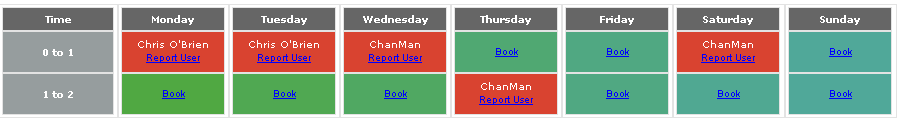
\includegraphics[width=14cm]{timetable.png}
\end{center}
\caption{Timetable display within application}
\label{fig:timetablesite}
\end{figure}


\subsection{Tournaments and Timetable Events}

The third major area of the site were the \textit{Tournament} and \textit{Event} classes. The structure and configuration of these classes are not different from the \textit{User} or \textit{Timetable} classes. In the context of this report and application, an Event is any object that can populate a field within a Timetable class. 

\subsubsection{Events}

Within the scope of this application, an \textit{Event} is any item that can be scheduled within the Timetable object. As with the \textit{Tournament} class, the \textit{Event} class is configured much like the \textit{User} and \textit{Timetable} classes. One event that is required by all versions of the Timetable is the 'Free Court' event. This event is created by default (see Figure ~\ref{fig:createEvent}) either the first time an administrator attempts to create an Event, or to create a Timetable. An Event has two attributes: a name and an author. In the case of a system event, the name will be the login of the person who booked the timetable slot, while the author is defined as \textit{BOOKING SYSTEM}. For an administrator event, the name is defined by that administrator, while the author is listed as the administrator who created the event. Example events for Monaleen Tennis would be:

\begin{itemize}
\item Training Sessions
\item Club Social Events
\item Ladies Tennis
\item Recurring Tournaments
\item General Club Activities
\end{itemize}

\begin{lstlisting}
@RequestMapping(value = "/saveEvent", method = RequestMethod.POST)
public String saveEvent(Model model, @ModelAttribute("event") Event e,
	BindingResult result) {
	if (eventService.getEventById(1).equals(null)){
		e.setName("Free Court");
		e.setAuthor(userService.emailToName(SecurityContextHolder
		.getContext().getAuthentication().getName()));
		e.setEnabled(true);
		eventService.createEvent(e); // see Line 29-32 for creation of Event.
	}
	logger.info("Event Save Method....");
	if (result.hasErrors()) {
		return "createEvent";
	}
	if (eventService.exists(e.getName())) {
		result.rejectValue("name", "Duplicate Key",
		"This Event Name has already been used.");
		return "createEvent";
	} else {
		e.setAuthor(userService.emailToName(SecurityContextHolder
		.getContext().getAuthentication().getName()));
		e.setEnabled(false);
		eventService.createEvent(e);
		return viewEvent(model);
	}
}

//Event DAO 
public void createNewEvent(I_Event e){
	logger.info("Creating new event....");
	session().save(e);
}
\end{lstlisting}
\begin{figure}[H]
\caption{Event Creation}
\label{fig:createEvent}
\end{figure}

Lines 4 through 10 are necessary to ensure no NullPointerExceptions are introduced when creating a timetable. If no events exist within the system either the first time a timetable is created or, as illustrated above in Figure~\ref{fig:createEvent}, an event is created, the system will create a \textit{Free Court} event which is needed for the timetable to function correctly.

In order for an event to show up as an option when creating, or editing, a timetable, it must be enabled, as shown in Figure ~\ref{fig:enableEvent}. This implementation allows the administrator to pre-create events for later use without overcrowding the timetable.

\begin{lstlisting}
@RequestMapping("/changeEventStatus")
public String changeEventStatus(Model model, HttpServletRequest request) {
	Event e = (Event) eventService.getEventById(Integer.valueOf(request
	.getParameter("eventID")));
	if (e.isEnabled()) {
		e.setEnabled(false);
		eventService.updateEvent(e);
		return viewEvent(model);
	} else {
		e.setEnabled(true);
		eventService.updateEvent(e);
		return viewEvent(model);
	}
}
\end{lstlisting}
\begin{figure}[H]
\caption{Change Event Status}
\label{fig:enableEvent}
\end{figure} 	

\subsubsection{Tournament}

The \textit{Tournament} class is configured similar to the \textit{Timetable} class, in that it has a secondary table which contains a list of members who have registered for the tournament. The key area for tournament implementation was for the application to differentiate between the various states of the tournament, such as registration being enabled, yet the tournament not having started yet. It was also important that the tournament could link up with the Timetable system, in order to book slots to play the tournament. In this regards, a tournament was required to manage an Event object, see Figure ~\ref{fig:tourCreate}, and to ensure that no ambiguity was present when dealing with multiple tournaments and possible multiple timetables. It was also necessary for a Tournament object to manage its own event in order to minimise both the risk of ambiguity and administration involvement.

\begin{lstlisting}
@RequestMapping(value = "/registerTournament", method = RequestMethod.POST)
public String doCreateTournament(
	Model model, BindingResult result,
	@Validated(FormValidationGroup.class) @ModelAttribute("tournament") Tournament t) {
	
	if (result.hasErrors()) {
		return "createTournament";
	} 
	if (tournamentService.exists(t.getTournamentName())){
		if (eventService.exists(t.getTournamentName())){
		result.rejectValue("tournamentName", "Duplicate Key",
		"An event of this name already exists");
		return "createTournament";
	}
	result.rejectValue("tournamentName", "Duplicate Key",
		"A tournament of this name already exists");
		return "createTournament";
		}
	else {
		try {
			tournamentService.create(t);
			eventCreation(t);
			logger.info("Tournament Created");
			return "tournamentSuccess";
		} catch (Exception e) {
		return "error";
	}
}
public void eventCreation(Tournament t){
	Event e = new Event();
	e.setName(t.getTournamentName());
	e.setAuthor(userService.emailToName(SecurityContextHolder.getContext()
	.getAuthentication().getName()));
	eventService.createEvent(e);
}
\end{lstlisting}
\begin{figure}[H]
\caption{Tournament Creation}
\label{fig:tourCreate}
\end{figure}

Deleting a tournament needed similar logic, as displayed in Figure ~\ref{fig:deleteTour}. Similar to the \textit{User} class, the Tournament name, much like the username, is used as a primary key, and can be recycled once a tournament is deleted. 

\begin{lstlisting}
	@RequestMapping("/confirmDelete")
	public String deleteTournament(Model model, HttpServletRequest request){
		Tournament t = tournamentService.getTournamentById(request
				.getParameter("tournamentID"));
		tournamentService.deleteTournament(t);
		eventService.deleteEvent(eventService.getEventIdByName(t.getTournamentName()));
		model.addAttribute("tour", tournamentService.getAllTournaments());
		return "deleteTournament";
	}
\end{lstlisting}
\begin{figure}[H]
\caption{Delete Tournament}
\label{fig:deleteTour}
\end{figure}	

Due to constraints on time within the final year project, it wasn't possible to fully flesh out this area of the site, though it was implemented in such a way to allow for extensibility such as an interface for the sorting of registered members into teams. This interface would allow the specification of business logic to allow the system to, for example, sort tournament teams by experience and ranking.
	
\label{sec:adminImp}
\subsection{Administration - Security and Session Management}

The \textit{Administration} section of the application deals with the implementation, and configuration, of the security and session management aspects of the application. An administrator has the same structure as a \textit{User} and is defined by the \textit{Role} it has, as seen previously in Figure ~\ref{fig:secRoles}. These roles are configured through Spring Security, in which a specific database schema must be adhered to. By default, there should be two tables: \textit{users} and \textit{authorities}, with a foreign key constraint. In this application, as shown in Line 3, Figure ~\ref{fig:roleConfig}, this was modified to keep the user data within the same table.

\begin{lstlisting}
<security:authentication-provider>
<security:jdbc-user-service data-source-ref="dataSource"
id="jdbcUserService" authorities-by-username-query="select username, authority from users where binary username = ?" />
<security:password-encoder ref="passwordEncoder"></security:password-encoder>
</security:authentication-provider>
\end{lstlisting}
\begin{figure}[H]
\caption{Spring Role Configuration}
\label{fig:roleConfig}
\end{figure}

The security within the application is controlled by the \textit{security-context.xml} file, which used Expression Based Access Control [EBAC] in order to restrict site access to relevant roles. EBAC allows complicated boolean logic to be encapsulated within a single expression, such as whether a user is authenticated or not. The base class used within this application is \textit{SecurityExpressionRoot}. These expressions are contained within the \textit{security-context.xml} file, as seen in Figure ~\ref{fig:secContext}. This configuration file is partly responsible for controller access to the mappings within the application. 

\begin{lstlisting}
<security:http use-expressions="true">
<security:intercept-url pattern="/static/**" access="permitAll" />
<security:intercept-url pattern="/images/**" access="permitAll" />
<security:intercept-url pattern="/createmembers" access="permitAll" />
<security:intercept-url pattern="/tournamentSuccess" access="hasAnyRole('ROLE_ADMIN', 'ROLE_COMMITTEE')" />
<security:intercept-url pattern="/createNews" access="hasAnyRole('ROLE_ADMIN', 'ROLE_COMMITTEE')" />
<security:intercept-url pattern="/members" access="isAuthenticated()" />
</security:http>
\end{lstlisting}
\begin{figure}[H]
\caption{Security Context File Excerpt}
\label{fig:secContext}
\end{figure}

An issue that arises with this implement ion is that all resources, such as images, would automatically be blocked from appearing on the site unless explicitly defined. In the case of images, this would be very time consuming, especially when new images are added to the application frequently. In order to overcome this, Lines 2 and 3 are implemented. This syntax specifies that all files and folders within the \textit{static} and \textit{images} folder are to be granted access to all pages within the application. Site access can also be granted on an authentication basis, rather than a role based system, and this is implemented as show in Line 7 of Figure~\ref{fig:secContext}.

In addition to the expression level security, service-level security annotations are also in place. This gives the application an extra layer of security, as it restricts the use of methods within the service layer to defined roles. It is possible to use either expression level security or service level security independently. This is configured within the \textit{security-context.xml} file, Figure ~\ref{fig:secAnnotate}, and is implemented, as shown in Figure ~\ref{fig:secAnonImpl}, within the service layer. These annotation use the same roles as defined previously within the application. 

\begin{lstlisting}
<security:global-method-security secured-annotations="enabled"></security:global-method-security>
\end{lstlisting}
\begin{figure}[H]
\caption{Security Context Service Layer Annotation Configuration}
\label{fig:secAnnotate}
\end{figure}

\begin{lstlisting}
@Service("timetableService")
public class TimetableService {

private TimetableDAO timetableDAO;

	@Autowired
	public void setTimetableDAO(TimetableDAO timetableDAO) {
		this.timetableDAO = timetableDAO;
	}
	
	@Secured("ROLE_ADMIN")
	public void create(Timetable t){
		timetableDAO.createTimetable(t);
	}
	
	@Secured({"ROLE_ADMIN", "ROLE_MEMBER", "ROLE_COMMITTEE", "ROLE_WARNING", "ROLE_SUSPEND"})
	public void update(Timetable t){
		timetableDAO.updateTimetable(t);
	}
	
	public List<Timetable> getAllTimetables(){
		return timetableDAO.listTimetables();
	}
}
\end{lstlisting}
\begin{figure}[H]
\caption{Security Context Service Layer Annotation Implementation}
\label{fig:secAnonImpl}
\end{figure}

In the implementation shown above, there are some items to note: the \textit{Service} and \textit{Autowired} annotations. The \textit{Service} annotation allows implementation classes to be auto-detected through class-path scanning. The package that contains the Service classes is defined within another XML file, \textit{service-context.xml} within this application, Figure ~\ref{fig:serviceContext}. This file configures Spring to look for Service classes via annotations, and where to look for them.

\begin{lstlisting}
<context:annotation-config></context:annotation-config>
<context:component-scan base-package="service"></context:component-scan>
\end{lstlisting}
\begin{figure}[H]
\caption{Service Context Configuration}
\label{fig:serviceContext}
\end{figure}

The \textit{Autowired} annotation is used within the framework to mark a constructor or setter. Spring then passes the needed dependencies into the application with its dependency injection facilities. 

\section{Model View Controller}
\subsection{Controller Layer}

A Controller is a class within the application that creates and modifies a model, and passes it onto a View. A View will also pass information to a Controller, which will communicate with the Service layer to persist any relevant data within the application.

A Controller is annotated, as illustrated in Figure~\ref{fig:controller}, Line 1. This allows the DispatcherServlet to identify the controllers and inject them into the application. This behaviour is displayed in Figure~\ref{fig:dscomponent}, which shows the DispatcherServlet being configured to scan the controllers package looking for annotations.

\begin{lstlisting}
@Controller
public class TimetableController {
	//.........
}
\end{lstlisting}
\begin{figure}[H]
\caption{Service Context Configuration}
\label{fig:controller}
\end{figure}

\begin{lstlisting}
<context:component-scan base-package="controllers, email"></context:component-scan>
<mvc:annotation-driven></mvc:annotation-driven>
\end{lstlisting}
\begin{figure}[H]
\caption{Service Context Configuration}
\label{fig:dscomponent}
\end{figure}

In order for the application to choose the correct method within a specific controller, it is necessary to define a mapping. The \textit{RequestMapping} annotation is used for this purpose. This annotation maps a web request onto a handler method within a controller, as depicted in Figure~\ref{fig:requestmapping}. It is also important, within the scope of the Spring Security configuration, to ensure that this mapping has access rights defined within the application or access will be denied.

\begin{lstlisting}
@RequestMapping("/")
public String showHome(Model model) {
	logger.info("Showing Home Page....");
	News news = newsService.getLatestStory();
	model.addAttribute("newsHeader", news.getSummary());
	model.addAttribute("newsContent", news.getContent());
	return "index";
}
\end{lstlisting}
\begin{figure}[H]
\caption{Request Mapping}
\label{fig:requestmapping}
\end{figure}

This mapping responds to a request with the value '/', Line 1. On Tomcat servers, this the home page, as the URL will be \textit{localhost:8080/<application-name>/}. In this example, the latest news story is retrieved on Line 4, and values from it are added to the model displayed on the returned view.

Any value specified after \textit{localhost:8080/<application-name>/} will search for a mapping within all controllers in the application. If a mapping does not exist, a resource not found will be displayed. This is default behaeviour for a denied access attempt. In order to ensure the site can deal with invalid requests, an access denied handler can be defined within the Spring Security context file, as depicted in Figure~\ref{fig:accessDenied}. This allows a mapping to be specified for invalid requests,

\begin{lstlisting}
<security:access-denied-handler error-page="/denied" />
\end{lstlisting}
\begin{figure}[H]
\caption{Access denied Handler}
\label{fig:accessDenied}
\end{figure}

In this example, the \textit{denied} mapping, shown in Figure~\ref{fig:deniedMapping} is called, and the corresponding view displayed. 

\begin{lstlisting}
@RequestMapping("/denied")
public String showDeny(Model model){
	model.addAttribute("message", "The page you are looking for either does not exist, or you do not have access. Please contact an administrator if you believe this is an error.");
return "error";
}

//Error Page

<center>${message}</center>
\end{lstlisting}
\begin{figure}[H]
\caption{Error Page Mapping}
\label{fig:accessDenied}
\end{figure}

Line 3 shows a message being added to a model, which is added to a standard error page. This message will change depending on what error is being caught by the application. The message is then displayed by the 'error' View for the user, and the site appearance is not disrupted by a generic error page.

\subsection{Models within the Spring MVC Framework}

A model is a map containing a key-value pair that can be modified by a Controller and displayed by a View. A model is implicitly created by the framework by including a reference to it within the method signature in a controller, as illustrated in Figure~\ref{fig:modelDefine}. The below example adds two lists to a model: a list of disabled events and a list of enabled events, shown in Lines 5 and 6. The Controller then returns the value \textit{viewEvents} to the ViewResolver. The ViewResolver displays the relevant page that displays the information held within the model for the user, as depicted in Figure~\ref{fig:modelJSP}

\begin{figure}[H]
\begin{lstlisting}
@RequestMapping("/viewEvents")
public String viewEvent(Model model) {
	List<Event> eventsDisabled = eventService.listDisabledEvents();
	List<Event> eventsEnabled = eventService.listEnabledEvents();
	model.addAttribute("eventsEnabled", eventsEnabled);
	model.addAttribute("eventsDisabled", eventsDisabled);
    return "viewEvents";
	}
\end{lstlisting}
\caption{Model Definition}
\label{fig:modelDefine}
\end{figure}

\begin{figure}[H]
\begin{lstlisting}
<c:if test="${not empty eventsEnabled }">
<table class="members" align="center">
<tr><th>Enabled Events</th></tr>
<tr>
<th>ID</th><th>Name</th><th>Author</th><th>Action</th></tr>
<c:forEach var="row" items="${eventsEnabled}">
<sf:form method="post"
action="${pageContext.request.contextPath}/changeEventStatus"
commandName="eventsEnabled">
<tr>
	<td><input type="hidden" value="${row.id}" name="eventID" />${row.id}</td>
	<td>${row.name}</td>
	<td>${row.author}</td>
	<td><input value="Disable" type="submit" name="${row.id}" />
</sf:form>
</c:forEach>
</table>
<center><font color="red">${message }</font></center>
</c:if>
\end{lstlisting}
\caption{JSP View of model}
\label{fig:modelJSP}
\end{figure}

The page contains a conditional loop, Line 1, that checks if the model attribute, eventsEnabled, is empty. In the event that it is not, it will create a table to display the information to the user, as shown in Lines 2 through 17. The \textit{c:forEach} tag is the JSTL version of a for loop, which will be looked at in a later section. Line 18 is a message, that will display if the value is not null. This is used to display a confirmation or error message to the user when an action is performed on an event. An example would be an attempt to disable the \textit{Free Court} event. This will display a message, shown below in Figure~\ref{fig:modelFail}, that the action cannot be performed.

\begin{figure}[H]
\begin{lstlisting}
if (e.getName().equalsIgnoreCase("Free Court")){
	model.addAttribute("message", "You cannot modify the Free Court event");
	return viewEvent(model);
}
\end{lstlisting}
\caption{User message added to model}
\label{fig:modelFail}
\end{figure}

\subsection{View Layer}
\subsubsection{Apache Tiles Configuration and Implementation}
Apache Tiles is configured within the web application core XML file. There are two classes that the configuration is concerned with: TilesViewResolver and TileConfigurer. Both are declared as beans within the configuration file and automatically created when the application is launched. The primary function of the ViewResolver is to take in a String value, and return the relevant \textit{RequestMapping} value within the application. These mappings are defined within the Controller classes of the application. The TilesConfigurer object, see Figure ~\ref{fig:tilesXML}, takes one parameter: a location of the template that the default tile will use. The default tile will then be used by other pages as a template. \newline

\begin{figure}[H]
\begin{lstlisting}
<bean id="tilesViewResolver"
	class="org.springframework.web.servlet.view.tiles2.TilesViewResolver">
</bean>

<bean id="tilesConfig"
	class="org.springframework.web.servlet.view.tiles2.TilesConfigurer">
	<property name="definitions">
	<list>
		<value>/WEB-INF/layout/default.xml</value>
	</list>
	</property>
</bean>
\end{lstlisting}
\caption{Apache Tiles Configuration}
\label{fig:tilesXML}
\end{figure}

The default tile consists of a number of sections identified by a specific tag. These tags correspond to values within the tile layout configuration file. Using a version of inheritance, these can be overwritten and replaced with other pages in order to change the content of a page, while maintaining cohesion across the design of the application. 

The following examples shows the implementation within the configuration file. The first section of code is the overall template. This specifies the default values that make up a JSP page within the application. The second segment of code is the the definition for the initial home page for the web application. By the inclusion of the \textit{extends="users.base"} within the definition tags, it is defining the index as a sub class of the users.base definition. Consequently, it is possible to override any of the attributes within the users.base definition. In this example, the title and content of the default page are being overridden with different values in order construct a more suitable page. The header, links and footer however remain the same, and will do so will all pages following this format, as shown in Figure ~\ref{fig:tilesConfig}.

\begin{figure}[H]
\begin{lstlisting}
<definition name="users.base" template="/WEB-INF/templates/default.jsp">
	<put-attribute name="title" value="Monaleen Tennis Club - Default Template"></put-attribute>
	<put-attribute name="header" value="/WEB-INF/tiles/header.jsp"></put-attribute>
	<put-attribute name="links" value="/WEB-INF/tiles/links.jsp"></put-attribute>
	<put-attribute name="content" value="/WEB-INF/tiles/content.jsp"></put-attribute>
	<put-attribute name="footer" value="/WEB-INF/tiles/footer.jsp"></put-attribute>
</definition>

<definition name="index" extends="users.base">
	<put-attribute name="title" value="Monaleen Tennis Club - Home Page"></put-attribute>
	<put-attribute name="content" value="/WEB-INF/tiles/index.jsp"></put-attribute>
</definition>

<definition name="admin" extends="users.base">
	<put-attribute name="title" value="Monaleen Tennis Club - Admin"></put-attribute>
	<put-attribute name="content" value="/WEB-INF/tiles/admin.jsp"></put-attribute>
</definition>
\end{lstlisting}
\caption{Apache Tiles Configuration}
\label{fig:tilesConfig}
\end{figure}

\subsubsection{JSTL}

JSTL is used within the application to manage how information was displayed. It was preferred, during the development of the application, that all of the logic be handled at the Controller level, and that the JSP pages would resolve the models passed to it into the view seen by the user. It was not desirable for the pages to contain JSP directives, or to use the implicit objects contained within JSP pages. 

The main tags used within the application were the JSTL Core tags.  These tags allow the usage of conditional statements and the definition of parameters within the JSP page. In order to use this technology, the relevant jar must be made available in the build path or within the Maven dependencies of the project. A declaration, as shown in Figure ~\ref{fig:jstldec} must be included in all JSP pages that wish to make use of the tags also.\newline

\begin{figure}[H]
\begin{lstlisting}
<%@ taglib prefix="c" uri="http://java.sun.com/jsp/jstl/core"%>
\end{lstlisting}
\caption{JSTL Tag Library Declaration}
\label{fig:jstldec}
\end{figure}

Within the application, the controller will create a model and pass it to the JSP page. The page uses the JSTL tags to manage and display relevant information from the model, as shown in Figure ~\ref{fig:ttmodelattributes}, and user actions based on the information contained within. The example below is taken from the Timetable display page, Figure ~\ref{fig:ttcontrollerchoosecourt} from the application.\newline

\begin{lstlisting}
@RequestMapping(value = "/gotoCourt", method = RequestMethod.POST)
public String chooseCourt(Model model, HttpServletRequest request) {
	//abbreviated method to display court, logic removed
	//highlighting the attributes within the model
	model = addDateToTimetable(model, id));
	model.addAttribute("series",timetableService.getById(id).getSeries());
	model.addAttribute("name", SecurityContextHolder.getContext().getAuthentication().getName());
	model.addAttribute("court", current);
	model.addAttribute("realname", name);
	model.addAttribute("bookings", left);
	if (seriesMatch(courtID, nextCourt)) {
		model.addAttribute("next", (current.getId() + 1));
	}
	if (seriesMatch(courtID, prevCourt)) {
		model.addAttribute("prev", (current.getId() - 1));
	}
	return "court";
}
\end{lstlisting}	
\begin{figure}[H]
\caption{Timetable Controller chooseCourt() method}
\label{fig:ttcontrollerchoosecourt}
\end{figure}

\begin{table}[H]
\begin{center}
\caption{Model Attributes}
    \begin{tabular}{ | l | l | p{5cm} |}
    \hline
    Model Name & Summary \\ \hline
    name & The username of the currently authenticated user  \\ \hline
    realName & The real name of the currently authenticated user\\ \hline
	bookings & The number of remaining bookings of the currently authenticated users\\ \hline
	date & The current week of the year and the current date. Calculated using separate method.\\ \hline
	next & The id number of the court following the current court, if applicable\\ \hline
    prev & The id number of the court preceding the current court, if applicable\\ \hline
	court & The current court, determined by the current week, provided by the java.util.Date class \\
    \hline
    \end{tabular}
\end{center}

\label{fig:ttmodelattributes}
\end{table}


This example is an excerpt from the TimetableContoller class. The logic determining the values has been removed. This is to highlight how attributes are added to the model from within the controller. This is the information that the JSP page will have access to once it has been displayed.

The above code deals with the display of \textit{Monday} within the Timetable display page. In the \textit{c:forEach} tags, it loops through each value in the \textit{court.monday} list that has been passed to it by the controller. The size of this list is determined by the user when the timetable is created, and the number of slots per day is specified. If the current value being examined in the loop is equal to the value "Free Court", it will display a link to the Book Form mapping. This aspect of the Timetable Controller will check that a user has any remaining bookings left and respond as appropriate. In the event that the value in the list does not equal "Free Court", it will make a choice. If the currently authenticated user made the booking, it will display an option to remove their booking from the slot. Otherwise, it will give any other user an option to report the user as a "no show" should a user fail to show for a previously booked slot. \newline

\begin{figure}[H]
\begin{lstlisting}
<c:forEach var="row" varStatus="loop" items="${court.monday}">
<c:choose>
<c:when test='${row eq "Free Court"}'><tr>
<td class="inner"><form action="${pageContext.request.contextPath}/bookCourt"
method="POST">
<input type="hidden" value="${loop.index}" name="position" />
<input type="hidden" value="monday" name="day" /> 
<input type="hidden" value="${court.id }" name="ttid" />
<input type="submit" value="Book">
</form></td></tr>
</c:when>
<c:otherwise><tr><td class="inner">${row}
<c:choose>
<c:when test="${name eq pageContext['request'].userPrincipal.name && row eq realname }">
<form action="${pageContext.request.contextPath}/unbookCourt" method="POST">
<input type="hidden" value="${loop.index}" name="position" />
<input type="hidden" value="monday" name="day" /> 
<input type="hidden" value="${court.id }" name="ttid" /> 
<input type="submit" value="Unbook">
</form></c:when>
<c:otherwise>
<form action="${pageContext.request.contextPath}/reportNoShow" method="POST">
<input type="hidden" value="${row}" name="bookedUser" />
<input type="hidden" value="monday" name="day" /> 
<input type="hidden" value="${court.id }" name="ttid" /> 
<input type="submit" value="Report User">
</form></c:otherwise>
\end{lstlisting}
\caption{Code Showing Display of Timetable}
\end{figure}


\section{Logging the Application}

The logging for this application was provided by \textit{log4j.} Logging became very useful for tracking down, and isolating bugs, throughout the application. Since there were a considerable number of dependencies and different technologies working together, it rapidly became very difficult to see where errors originated from. Stack-traces quickly became unmanageable. \textit{Log4j} works by allowing the developer to view a number of logs of varying types within the application.
\begin{table}[H]
\caption{Log Types}
\begin{center}
    \begin{tabular}{ | l | l | p{5cm} |}
    \hline
    Log Type & Description \\ \hline
    INFO & Messages that highlight the progress of the application at coarse-grained level  \\ \hline
    DEBUG & Fine-grained informational events that are most useful to debug an application\\ \hline
	TRACE & Finer-grained informational events than the DEBUG\\ \hline
	WARN & Potentially harmful situations\\ \hline
	ERROR & Error events that might still allow the application to continue running\\ \hline
    FATAL & Very severe error events that will presumably lead the application to abort\\ \hline
    \end{tabular}
\end{center}

\end{table}

\textit{Log4j} is configured with a properties file that allows you to see the various levels of logs displays by the applications running. Implementation of a logging system resolved a number of Spring Security issues within the web application. Spring Security, concerned with access rights to mappings within the application, did not output failed access attempts to the console. This made it very difficult to debug. When configuring \textit{Log4j} to catch the logs created by the security components, the application became much easier to debug. The properties file for this web application is detailed below.

\begin{figure}[H]
\begin{lstlisting}
log4j.rootLogger=INFO, CONSOLE
log4j.appender.CONSOLE=org.apache.log4j.ConsoleAppender
log4j.appender.CONSOLE.layout=org.apache.log4j.SimpleLayout
log4j.logger.org.hibernate.SQL=DEBUG
log4j.logger.org.hibernate.type=TRACE
log4j.logger.org.springframework.security=DEBUG
\end{lstlisting}
\caption{Log4j Configuration}
\end{figure}

Logging can be implemented on a class by class basis. Within this application, it was used to display informational messages to the developer. These included items such as database access, objects being created and updated. In order to enable logging on a class, a logger must be instantiated with reference to the class that requires logging. The logger object then is called with a method corresponding to the type of log you wish to throw along with a message.

\begin{figure}[H]
\begin{lstlisting}
private static Logger logger = Logger.getLogger(UserDAO.class);

public Session session(){ 
	logger.info("Session Factory returning current session.....");
	return sessionFactory.getCurrentSession();
}

public List<User> getUsers() {
	logger.info("Selecting All Enabled Members....");
	return session().createQuery("from User where enabled = '1'").list();
}

public User getUserByName(String name) {
	Criteria crit = session().createCriteria(User.class);
	crit.add(Restrictions.eq("name", name)); 
	try{
	User user = (User) crit.uniqueResult();
	}
	catch(Exception e){
	logger.error{"Must be unique result : Thrown from UserDAO.getUserByName(String name));
	}
	return user;
}
\end{lstlisting}
\caption{Logger Usage within UserDAO.class}
\end{figure}

\section{Configuration of the Application}

In order to begin implementation with the Spring MVC framework, there are a number of configuration files that are necessary. The core file is the \textit{web.xml} file. This file is responsible for the configuration for the framework. One of the key responsibilities is the definition of the context xml files, whose purpose will be elaborated on later. Different development profiles can be configured within this file in order to produce different development environments, such as production and testing environments. The configuration of this file within the application is shown in Figure ~\ref{fig:springConfig} \newline 
\begin{figure}[H]
\begin{lstlisting}
<context-param>
<param-name>contextConfigLocation</param-name>
<param-value>
	classpath:beans/dao-context.xml
	classpath:beans/service-context.xml
	classpath:beans/security-context.xml
</param-value>
 </context-param>
\end{lstlisting}
\caption{Spring Configuration}
\label{fig:springConfig}
\end{figure}

Of particular importance are the definition of the context parameters. In this project, there were three main context files.

\begin{itemize}
\item Data Access Object Context
\item Service Context
\item Security Context
\end{itemize}

The DAO Context file specifies the packages that contain the various DAO classes within the application. It also contains configurations for both the database connection details, and Hibernate configurations. Packages containing entity classes for Hibernate are specified within this context also. \newline

\begin{figure}
\begin{lstlisting}
<property name="hibernateProperties">
<props>
<prop key="hibernate.dialect">org.hibernate.dialect.MySQL5Dialect</prop>
</props>
</property>
\end{lstlisting}
\caption{Hibernate Configuration}
\end{figure}


The Service Context file is responsible for specifying the base package containing the Service classes necessary to facilitate the collaboration between the Controller classes and the DAO classes. This file specifies that annotations will be used to configure the Service classes.\newline
\begin{figure}
\begin{lstlisting}
<context:annotation-config></context:annotation-config>
<context:component-scan base-package="service"></context:component-scan>
\end{lstlisting}
\caption{Service Context Configuration}
\end{figure}

The Security Context file is the larger of the three files, and is responsible for the security configuration of the web application. There are four main areas within the file that were used to configure the web application created in this project. \newline The User Service aspect of the configuration file is responsible for retrieving users and their authority within the scope of the web application. \newline The URL access configuration ensures that only users who are authorised to access certain portions of the site are allowed access. \newline The Security Annotations allow the creation of an extra level of security into an application. At class level, annotations can be placed on methods to further ensure that proper access is enforced throughout the application. \newline Lastly, the Security Context is responsible for creating the password encoder bean in which passwords are encoded, and decoded, upon account creation and login. This ensures that no passwords in plain text form are ever stored on either the server or the database within the web application \pagebreak

\begin{itemize}
\item User Service
\begin{lstlisting}
<security:authentication-manager>	
	<security:authentication-provider>
	<security:jdbc-user-service data-source-ref="dataSource"
		id="jdbcUserService" authorities-by-username-query="select username, authority from users where binary username = ?" />
	<security:password-encoder ref="passwordEncoder"></security:password-encoder>
	</security:authentication-provider>
</security:authentication-manager>
\end{lstlisting}
\item URL Access
\begin{lstlisting}
<security:intercept-url pattern="/timetable" access="permitAll"/>
<security:intercept-url pattern="/reportNoShow" access="permitAll"/>
<security:intercept-url pattern="/admin" access="hasRole('ROLE_ADMIN')"/>
<security:intercept-url pattern="/approveMembers" access="hasRole('ROLE_ADMIN')"/>
\end{lstlisting}
\item Security Annotation for Service Class
\begin{lstlisting}
<security:global-method-security secured-annotations="enabled"></security:global-method-security>
//Java Code from TimetableService class. 
//This code is invoked when booking a slot on the timetable and is only accessible by registered members.
@Secured({"ROLE_ADMIN", "ROLE_MEMBER", "ROLE_COMMITTEE", "ROLE_WARNING", "ROLE_SUSPEND"})
	public void update(Timetable t){
		timetableDAO.updateTimetable(t);
	}
\end{lstlisting}
\item Password Encoding
\begin{lstlisting}
<bean id="passwordEncoder"
class="org.springframework.security.crypto.password.StandardPasswordEncoder">
</bean>
\end{lstlisting}
\end{itemize}

\section{Test Driven Development}

The primary method of testing was implemented using JUnit. A Test Suite of JUnit tests were prepared to test the key features of the application. A separate test database was constructed. It was important to ensure that the testing environment was using the same context files as the production environment. The test class had to be annotated to enforce this. While the context files were the same, the DataSource file has changed as a different database is being using in this environment.


\begin{figure}[H]
\begin{lstlisting}
@ActiveProfiles("dev")
@ContextConfiguration(locations = { "file:src/main/java/beans/dao-context.xml",
"file:src/main/java/beans/security-context.xml",
"classpath:test/config/datasource.xml" })
@RunWith(SpringJUnit4ClassRunner.class)
public class HibernateTests {
	
	@Autowired
	private UserDAO userDAO;
	
	@Autowired
	private TournamentDAO tournamentDAO;
	
	@Autowired
	private DataSource dataSource;
	
	//Class truncated 
}

\end{lstlisting}
\caption{JUnit Test Example}
\end{figure}

The database is then initialised to ensure the tests are being run against the same database, and that repeat tests are consistent.

\begin{figure}[H]
\begin{lstlisting}
@Before
public void init(){
	JdbcTemplate jdbc = new JdbcTemplate(dataSource);
	jdbc.execute("delete from users"); 
}
\end{lstlisting}
\caption{JUnit @Before Test Configuration}
\end{figure}

In these example tests, the UserDAO is being tested to ensure that it returns true when the exists() method is called on it. This is important within the scope of the application to ensure that primary keys are not duplicated. The method is annotated with \textit{@Test}. The methods \textit{assertTrue} and \textit{assertFalse} expect a return value of true and false respectively. They take two parameters: an error message and a boolean value, or a method that returns a boolean value. In the \textit{assertTrue} method below, the UserDAO will return true if the user exists. In the event that the user does not exist, it will fail the test and return the message "User should exist".\newline 

\begin{figure}[H]
\begin{lstlisting}
@Test
public void testExists(){
	userDAO.createUser(user1);
	assertTrue("User should exist", userDAO.exists(user1.getUsername()));
	assertFalse("User should not exist", userDAO.exists("jkljfksakfjahghdsopjclkhfkjafhkjdshFHajhgouwe"));
}
\end{lstlisting}
\caption{JUnit UserDAO Exists() Test}
\end{figure}

Another test with the UserDAO was to ensure that users were being saved correctly. In this example, users are being created and saved to the database. The method \textit{assertEquals} checks two interger values and returns an error message if they do not match.

\begin{figure}[H]
\begin{lstlisting}
@Test 
public void testCreateRetrieve(){
	userDAO.createUser(user1);
	List<User> users1 = userDAO.getAllUsers();
	assertEquals("One user should have been created and retrieved", 1, users1.size());
	assertEquals("Inserted user should match retrieved", user1, users1.get(0));
	userDAO.createUser(user2);
	userDAO.createUser(user3);
	userDAO.createUser(user4);
	List<User> users2 = userDAO.getAllUsers();
	assertEquals("Number of users should be four", 4, users2.size());
}
\end{lstlisting}
\caption{JUnit Create and Size Test}
\end{figure}

\section{External Code}
There are two aspects of external code being used within this web application. The first is the CSS file that the site is using. This was a free template obtained from \href{http://skylinestemplates.blogspot.ie/2011/11/greefies-solution-xhtml-and-css.html}{Skylines Templates}

This template was modified in order to fit in with certain aspects of the site, but the look, feel and images remain consistent with those of the template.

The other code used in this application that was not original is the Google Maps script, visible in the Contact Us page of the web application. This is provided at \href{https://developers.google.com/maps/documentation/javascript/examples/map-simple}{Google Maps Simple Map Example} and is available to use freely. The code was slightly modified, as depicted in Figure~\ref{fig:googlemaps}, to change both the GPS co-ordinates and the initial zoom level of the map. The page is included in the Contact Us tile.\newline

\begin{table}[H]
\begin{lstlisting}
//code to include maps.jsp in contactus.jsp
<div align="center"><%@include file="maps.jsp"%></div>

//code of the maps.jsp change with modified Google javascript
<script src="http://maps.googleapis.com/maps/api/js?sensor=false">
</script>
<script>
function initialize()
{
var mapProp = {
center:new google.maps.LatLng(52.6565176,-8.5537577), //GPS Co-ords
zoom:18, // Zoom level
mapTypeId:google.maps.MapTypeId.ROADMAP
};
var map=new google.maps.Map(document.getElementById("googleMap"),mapProp);
}
google.maps.event.addDomListener(window, 'load', initialize);
</script>

\end{lstlisting}
\caption{Code Showing Google Maps Integration}
\label{fig:googlemaps}
\end{table}

\section{Conclusion}

\chapter{Software Quality}
\label{squality}

\section{Application Summary}

(Discssion on software metrics)
- Software Metrics - A Rigorous Approach - Norman Fenton (ref)

The following is a summary of the various metrics of the application. A detailed breakdown by package in contained within the appendices.

\begin{table}[H]
\begin{center}
    \begin{tabular}{| l | l | l | l | p{2.3cm} |}
    \hline
    Metric & Total & Mean & Std. Deviation & Maximum\\ \hline
	McCabe Cyclomatic Complexity & n/a & 1.262 & .862 & 8\\ \hline
    
    \end{tabular}
\end{center}
\caption{Application Metrics}
\end{table}


\section{Software Quality Tools and Visualisations}

\begin{figure}[H]
\begin{center}
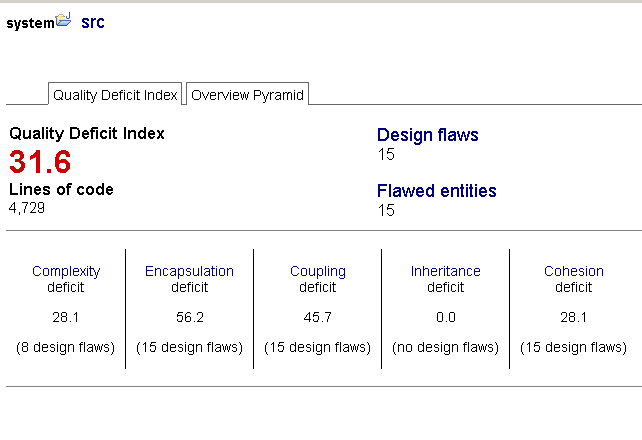
\includegraphics[scale=0.7]{infusion1.PNG}
\end{center}
\caption{Pre Re-factoring using Infusion}
\end{figure}

\begin{figure} [H]
\begin{center}
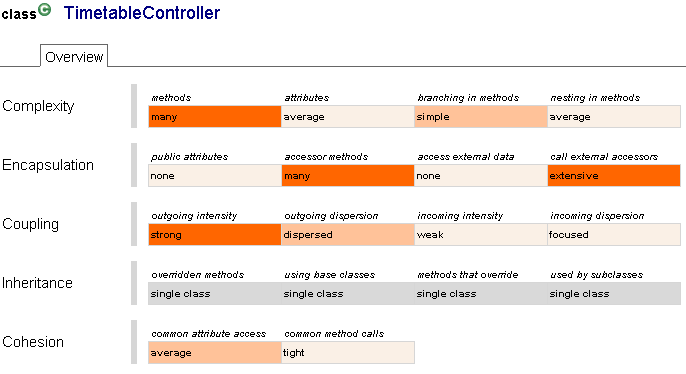
\includegraphics[scale=0.7]{infusion3.PNG}
\caption{Example of Class 'Bad Code Smell' Breakdown using Infusion}
\end{center}
\end{figure}

\begin{figure}[H]
\begin{center}
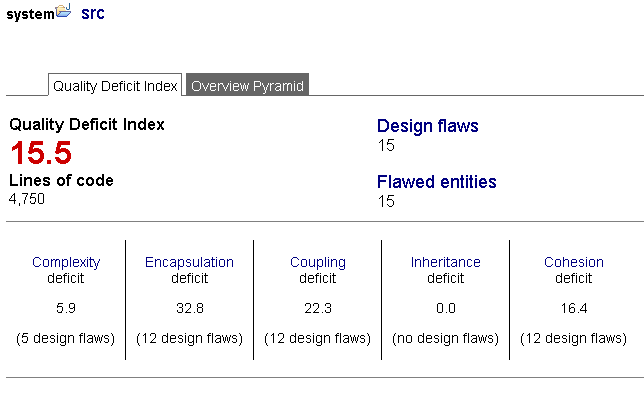
\includegraphics[scale=0.7]{infusion2.PNG}
\caption{Post Re-factoring using Infusion}
\end{center}
\end{figure}

\begin{figure}[H]
\begin{center}
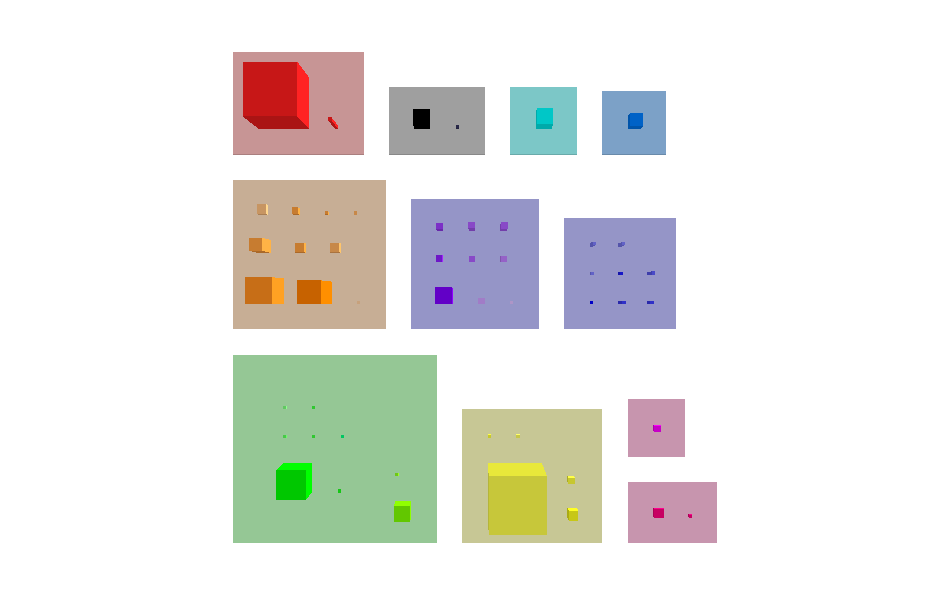
\includegraphics[scale=0.5]{codecity2d.png}
\caption{CodeCity 2D Visualisation of Application}
\end{center}
\end{figure}

\begin{figure}[H]
\begin{center}
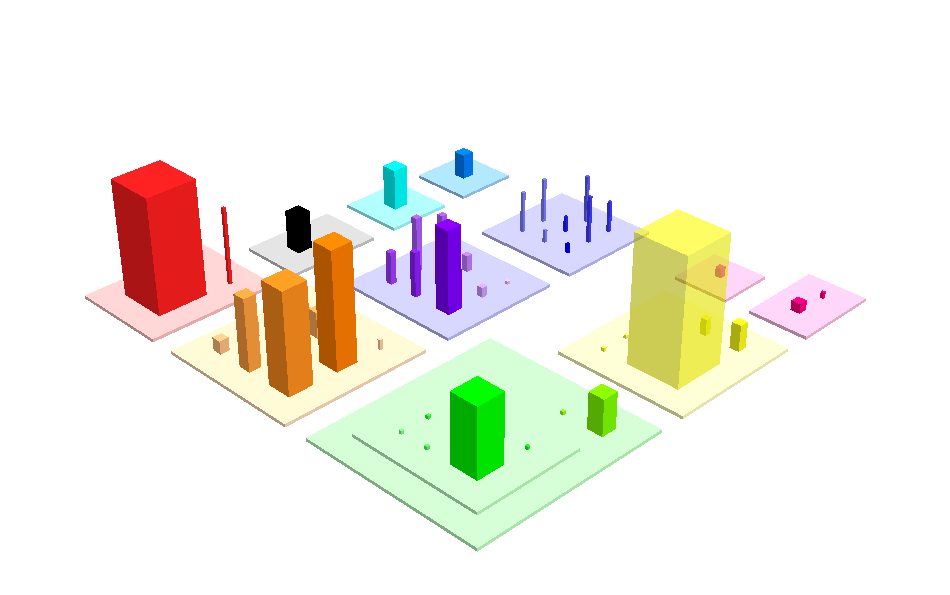
\includegraphics[scale=0.5]{codecity3d.png}
\caption{CodeCity 3D Visualisation of Application}
\end{center}
\end{figure}



\section{Sample Refactorings}

\chapter{Evaluation}
\label{evaluation}

\section{Security}

\subsection{OWASP Vulnerabilities}

In analysing support for security, the Open Web Application Security Project [OWASP] was examined. OWASP provides a list of the top 10 vulnerabilities that exist within web applications. The following vulnerabilities are addressed directly by the frameworks used in this project.

\begin{enumerate}
\item Injection
\begin{itemize}
\item Injection occurs when "untrusted data is sent to an interpreter as part of a command or query" \parencite{owasp2013}. This can allow unauthorised access to a database, and the exposure of the data within. Hibernate aids the prevention of Injection by providing support for named parameters. Hibernate further prevents injection by eliminating SQL queries entirely, and by creating objects through mapping of attributes to columns within the database. JDBC does not support the use of named parameters natively, but Spring does provided a \textit{NamedParameterJdbcTemplate} class which provides this functionality to the JDBC class. 

\end{itemize}

\item Broken Authentication and Session Management
\begin{itemize}
\item This occurs when "application functions related to authentication and session management are often not implemented correctly" \parencite{owasp2013}. When developers create their own session management schemes, they will inadvertently introduce flaws. Spring provides robust session management and authentication techniques through the use of EBAC, as discussed earlier. This allows the developer to focus more on the design of the application, and the business logic within, without having to be concerned with created a strong security solution.
\end{itemize}

\item Cross Site Scripting (XSS)
\begin{itemize}
\item XSS is "whenever an application takes untrusted data and sends it to a web browser without proper validation or escaping" \parencite{owasp2013}. This allows the potential use of malicious scripts in a victims browser, which may enable an attacker to gain access to the user session. Spring provides an extension of the Java EE 6 class \textit{HttpServletRequestWrapper} called \textit{XSSWrapper}. This class takes a HTTP Request object, and checks the values of getParamters(), getParameterValues() and getHeaders(). The XSSWrapper object then performs a stripXSS() method that checked the validity of the parameters with an HttpServletRequest object, and in the event that an attempted XSS attack is present, nullifies it by escaping special characters.
\end{itemize}

\item Security Misconfiguration
\begin{itemize}
\item Security Misconfiguration is not "having a secure configuration defined and deployed for the application framework" \parencite{owasp2013}. Within Spring MVC, this refers to the configuration for EBAC. An example of poor configuration would be to implement this system by denying access to URL mappings, rather than denying access to all and allowing exceptions. While it is possible to deny access to relevant mappings, it is more likely that a mistake would slip through. A breakdown of the mappings organised by the type of access is depicted in Table~\ref{fig:accesstable}. permitAll refers to mappings that allow access to all users, isAuthenticated requires that the user be logged in, and admin requires that a user be logged in and possess an administrator role.

\begin{table}[H]
\caption{EBAC Breakdown}
\begin{center}
    \begin{tabular}{ | l | l | l | p{5cm} |}
    \hline
	\textbf{permitAll} & \textbf{isAuthenticated}& \textbf{admin}\\ \hline
	23 & 13 & 50\\ \hline
    \end{tabular}
\end{center}
\label{fig:accesstable}
\end{table} 
\end{itemize}

\item Sensitive Data Exposure
\begin{itemize}
\item Sensitive Data Exposure deals with the encryption of sensitive user information such as passwords, credit card details and anything that made lead to identity theft. This data "deserves extra protection such as 
encryption at rest or in transit" \parencite{owasp2013}. Within the scope of this application, the main concern was user passwords, as no payment information is held. Spring provides methods for encoding data using 256bit AES encryption. The encrypted value is stored in the database, not the actual password. When the user logs in, the plaintext password is encrypted  using a key unique to that user. The encrypted password is then compared to the stored value. Each user has a unique key to generate the password so that even if two users have the same password, it will not appear the same in the stored values. 
\end{itemize}

\item Unvalidated Redirected and Forwards
\begin{itemize}
\item Within any web application, they will be scope for redirects. For example, if a user logs in, it is normal to redirect them to the home page. However, the application must be cognisant of where the redirect is coming from, and ensure its validity. "Without proper validation, attackers can redirect victims to phishing or malware sites, or use forwards to access unauthorized pages" \parencite{owasp2013}. The ViewResolver, provided in Spring and extended by Apache Tiles, is responsible for validating this information. All redirected are passed to the ViewResolver as a string. If a value corresponding to this string is not found within the ViewResolver configuration, an error will be returned in the form of a 404 Page Not Found value or an access denied value, as defined in the security-context file. 
\end{itemize}
\end{enumerate}

\subsection{Security Bugs}

A significant bug was discovered within the application during user testing. When a user was editing their profile, a model attribute was used to map the data changed in the View to create an object within the Controller. The application did not allow the user to edit all attributes within the user class, such as their role within the application. As a result, any changes to a user object where the attributes were not defined within the view resulted in attributes not present in the view being set as null. This meant that a user would have no role within the system, as the role attribute would be changed to null. To overcome this, a hidden value mapped to the role attribute was inserted into the form. This fixed the problem, but in doing so, introduced a significant security risk. 

Using a tool to intercept HTTP Requests, such as WebScarab, it was possible to change the hidden field. This would allow a regular user to change their role from ROLE MEMBER to ROLE ADMIN, giving them full access to the site. This happened as the object was not checked before being persisted by the controller, service and dao layers. This method was tested using the WebScarab tool, and the vulnerability was confirmed. WebScarab is a framework that analysing applications that communicate using HTTP and HTTPS protocols, and was used to intercept GET and POST requests in this application. In order to circumvent this, the role of the currently logged in user was retrieved from the framework, and this value was saved, rather than a value defined within the view. This example showed that while the framework does provide a considerable layer of security, misuse and bad programming can expose the application. 

\section{Extensibility}

The goal of extensibility is "controlling the time and costs to implement, tests and deploy changes" \parencite{bass2003software}. The use of Hibernate in the architectural stack provides a measure of extensibility support for changes in entity classes. Any addition to an entity class would result in a change to a database schema. 

An application using Hibernate, in conjunction with Spring MVC, would need only to modify the View, illustrated in Figure~\ref{fig:viewChange}. This would need to be changed to facilitate input of the new attribute. Spring MVC uses spring form tags to map values to the object within the Controller, and the DAO layer persists the object. Since the object is configured with database mapping at class level, no changes are necessary to the DAO. The addition of Line 14 is Figure~\ref{fig:viewChange} is the only changed needed to allow for the attribute to be modified within the application. The Controller, Service layer and DAO would remain unchanged.

\begin{table}[H]
\begin{lstlisting}
<sf:form id="details" method="post" action="${pageContext.request.contextPath}/adminProfileUpdate" commandName="member">
<table class="formtable">
Name:<sf:input name = "name" path="name" type="text"/>
Email:<sf:input name = "username" path="username" type="text"/>
Password:<sf:input name = "password" path="password" type="text"/>
Address Line 1<sf:input name = "ad_line1" path="ad_line1" type="text"/>
Address Line 2<sf:input name = "ad_line2" path="ad_line2" type="text"/>
City/Town<sf:input name = "ad_city" path="ad_city" type="text"/><br/>
County<sf:input name = "ad_county" path="ad_county" type="text"/><br/>
Contact Number<sf:input name = "contact_num" path="contact_num" type="text"/>
Emergency Contact Name<sf:input name = "em_con_name" path="em_con_name" type="text"/>
Emergency Contact Number<sf:input name = "em_con_num" path="em_con_num" type="text"/>
Role<sf:select path="authority"><sf:options items="${roles }"/></sf:select>
New Attribute<sf:input name = "new_attribute" path="new_attribute" type="text"/> //new line added
<input type="hidden" value="${member.username }" name="username"/>
<input value="Change Details" type="submit"/>
\end{lstlisting}
\caption{Change to view to support new attributes}
\label{fig:viewChange}
\end{table}
Using JDBC, again in partnership with Spring MVC, the View and the DAO object would need to be changed. Within the DAO, two actions must be performed, as depicted in Figure~\ref{fig:jdbcChanges}. Line 18 shows the addition of an extra parameter to map the value to a position in the SQL statement. The SQL statement must be modified also in order to correctly insert or update the persisted value in the database. This is shown in Lines 23 through 26, with the changes being shown in capital letters. 

\begin{lstlisting}
@Transactional
public boolean createUserJDBC(User user) {
MapSqlParameterSource params = new MapSqlParameterSource();
params.addValue("username", user.getUsername());
params.addValue("name", user.getName());
params.addValue("password", passwordEncoder.encode(user.getPassword()));
params.addValue("gender", user.getGender());
params.addValue("member_type", user.getMember_type());
params.addValue("grade", user.getGrade());
params.addValue("ad_line1", user.getAd_line1());
params.addValue("ad_line2", user.getAd_line2());
params.addValue("ad_city", user.getAd_city());
params.addValue("ad_county", user.getAd_county());
params.addValue("contact_num", user.getContact_num());
params.addValue("em_con_name", user.getEm_con_name());
params.addValue("em_con_num", user.getEm_con_num());
params.addValue("role", "ROLE_MEMBER");
params.addValue("NEW_ATTRIBUTE", "user.getNEW_ATTRIBUTE());
return jdbc
	.update("insert into users (username, name, password, gender, 
	member_type, grade, ad_line1, ad_line2, ad_city, ad_county,
	contact_num, em_con_name, em_con_num, enabled, authority,
	bookings_left, NEW_ATTRIBUTE) values (:username, :name, :password, 
	:gender, :member_type, :grade, :ad_line1, :ad_line1, 
	:ad_city, :ad_county, :contact_num,:em_con_name, :em_con_num,
	false, :role, 0, :NEW_ATTRIBUTE)",params) == 1;
	}
\end{lstlisting}
\begin{table}[H]
\caption{JDBC DAO changes with entity change}
\label{fig:jdbcChanges}
\end{table}

Hibernate provides better support for extensibility in this regard, allowing the developer to focus on database and view changes, with no need to modify the persistence layer between the application and the database.

\section{Usability}

The deliverable from this project was subjected to the same usability criteria as illustrated in Section~\ref{sec:usabilty}. The results are shown in Tables~\ref{fig:projecttable1} through~\ref{fig:projecttable5}. The overall results are compared in Figure~\ref{fig:projecttable6}.

\begin{table}[H]
\caption{Table 1 - Links}
\begin{center}
    \begin{tabular}{ | l | l | p{5cm} |}
    \hline
\textbf{Criteria} & \textbf{Project Application}\\ \hline
	Links are updated? & Yes\\ \hline
	Short-cuts for frequent users? & Yes\\ \hline
	Warning if link leads to large file? & n/a\\ \hline
	Indication of restricted access for link & Yes \\ \hline
	Link text indicates nature of target & Yes \\ \hline
	Total & 4/5 \\ \hline	
    \end{tabular}
\end{center}
\label{fig:projecttable1}
\end{table}

\begin{table}[H]
\caption{Table 2 - Feedback Mechanisms}
\begin{center}
    \begin{tabular}{ | l | l | p{5cm} |}
    \hline
\textbf{Criteria} & \textbf{Project Application}\\ \hline
	Contact Details for website maintainer & Yes \\ \hline
	Link to page maintainer on each page & Yes \\ \hline
	Forms provided for users to enter details & Yes\\ \hline
	FAQ provided & Yes \\ \hline
	Feedback mechanisms are fully operational & Yes\\ \hline
	Total & 5/5 \\ \hline	
    \end{tabular}
\end{center}
\label{fig:projecttable2}
\end{table}

\begin{table}[H]
\caption{Table 3 - Accessability}
\begin{center}
    \begin{tabular}{ | l | l | p{5cm} |}
    \hline
\textbf{Criteria} & \textbf{Project Application}\\ \hline
	Speed of site adequate& Yes\\ \hline
	Site Availability High? & Yes\\ \hline
	Website made known through search tools** & n/a \\ \hline
	Link back to parent entity & Yes\\ \hline	
	Name of entity reflected in URL & Yes \\ \hline	
	URL is not over complex,likely to be mistyped & Yes \\
	\hline	
	Total & 5/8\\ \hline	
    \end{tabular}
\end{center}
\label{fig:projecttable3}
\end{table}


\begin{table}[H]
\caption{Table 4 - Design}
\begin{center}
    \begin{tabular}{ | l | l | p{5cm} |}
    \hline
\textbf{Criteria} & \textbf{Project Application}\\ \hline
	Format,Graphic Design Appropriate & Yes \\ \hline
	Pages appropriate length, clear, uncluttered& Yes \\ \hline
	Consistent format through website & Yes \\ \hline
	Site compatible with multiple browsers & Yes\\ \hline
	Site can be used without graphics & No\\ \hline
	Total & 4/5 \\ \hline	
    \end{tabular}
\end{center}
\label{fig:projecttable4}
\end{table}

\begin{table}[H]
\caption{Table 5 - Navigability}
\begin{center}
    \begin{tabular}{ | l | l | p{5cm} |}
    \hline
	\textbf{Criteria} & \textbf{Project Application}\\ \hline
	Website organised by anticipated user need & Yes\\ \hline
	Navigation options are distinct& Yes \\ \hline
	Conventional navigation models*& Yes\\ \hline
	Navigation links are provided on all pages & Yes\\ \hline
	Browsing facilitated by menu or site map &Yes \\ \hline
	Reach any point in appropriate number of clicks** & Yes\\ \hline
	Search Engine Provided & No\\ \hline
	Total & 6/7 \\ \hline	
    \end{tabular}
\end{center}
\label{fig:projecttable5}
\end{table}
\textit{*eg menu on top or left of screen}\newline
\textit{**defined as 3,} \cite{smith2001applying}

\begin{table}[H]
\caption{Table 6 - Overall Results}
\begin{center}
    \begin{tabular}{ | l | l | p{5cm} |}
    \hline
	Site & Total\\ \hline
	Monaleen Tennis Club & 14/30\\ \hline
	Tralee Tennis Club & 22.5/30\\ \hline
	Project Application & 24/30\\ \hline	
    \end{tabular}
\end{center}
\label{fig:projecttable6}
\end{table}

\section{Productivity and Performance}

\subsection{Hibernate}

One of the core technologies used within the application was Hibernate. One of the main benefits Hibernate provided to the project was simplifying the code in order to persist objects. When developing the application, the only concern was with objects as a whole, not on their individual attributes. With JDBC, there was a need to use SQL syntax within the application. In the case of the User class, there were 16 attributes which made the SQL INSERT statement for that class, shown in Figure~\ref{fig:jdbcsql}, difficult to read and troubleshoot.

\begin{figure}[H]
\begin{lstlisting}
@Transactional
public boolean createUserJDBC(User user) {
	MapSqlParameterSource params = new MapSqlParameterSource();
		//other params cut out to save space
		params.addValue("role", "ROLE_MEMBER");
		return jdbc
			.update("insert into users (username, name, password, gender, 
			member_type, grade, ad_line1, ad_line2, ad_city, ad_county,
			contact_num, em_con_name, em_con_num, enabled, authority,
			bookings_left) values (:username, :name, :password, 
			:gender, :member_type, :grade, :ad_line1, :ad_line1, 
			:ad_city, :ad_county, :contact_num,:em_con_name, :em_con_num,
			false, :role, 0)",params) == 1;
	}
\end{lstlisting}
\caption{JDBC SQL INSERT}
\label{fig:jdbcsql}
\end{figure}

However, it could be arguing by supplying a framework, such as Hibernate, to automate the creation of a query language that performance of an application could be affected. To examine this briefly, a small test was created. This this test, the application would use JDBC to create 10,000 records, update those records and then delete them. The application would then perform the same actions with the same data using Hibernate. The time taken to perform these tasks as a whole would be recorded in nanoseconds. The test is illustrated in Figure~\ref{fig:jdbcvhibernate} below.

\begin{figure}[H]
\begin{lstlisting}
@RequestMapping("/testdatabases")
public String testdatabases(Model model){
	User user = new User(); // create a new user
	long jStart = System.nanoTime();
	model.addAttribute("jdbcStart", jStart);
	for (int i = 0; i < 10000; i++){
		user.setUsername(i + "@test.ie");
		userService.createJDBC(user);
		userService.enableUserJDBC(user);
		userService.deleteUserJDBC(user);
	}
	model.addAttribute("jdbcFinish", (System.nanoTime() - jStart));
	
	long hStart = System.nanoTime();
	model.addAttribute("hibernateStart", hStart);
	for (int i = 0; i < 10000; i++){
		user.setUsername(i + "@test.ie");
		userService.create(user);
		user.setEnabled(true);
		userService.updateUser(user);
		userService.delete(user);
	}
	model.addAttribute("hibernateFinish", (System.nanoTime() - hStart));
	return "testdatabases";
}
\end{lstlisting}
\caption{JDBC Vs Hibernate Test}
\label{fig:jdbcvhibernate}
\end{figure}

The results are displayed in Table~\ref{fig:resulttable} below. NS refers to NanoSeconds, and MM:SS refers to the total in minutes and seconds. The test was run three times and an average was created. The test machine was an Amazon EC-2 server, which was a 32-bit micro instance, with 650mb of RAM with one virtual CPU. This is running a modified version of Red Hat Enterprise Linux.

\begin{table}[H]
\caption{Hibernate Vs JDBC Results}
\begin{center}
    \begin{tabular}{ |l | l | l | l | p{2.5cm} |}
    \hline
     Run & Database & No Queries & Total (NS) & Total (MM:SS)\\ \hline
	 1 & Hibernate & 10,000 &198469890740&03:20\\ \hline
	 1 & JDBC & 10,000 &211883464327&03:30\\ \hline
	 2 & Hibernate & 10,000 &188055485374&03:07\\ \hline
	 2 & JDBC & 10,000 &200521721809&03:22\\ \hline
	 3 & Hibernate & 10,000 &188423897510&03:06\\ \hline
	 3 & JDBC & 10,000 &193541735201&03:20\\ \hline
	Avg & Hibernate & 10,000 &191649757878 &03:12\\ \hline
	Avg & JDBC & 10,000 & 201982307112&03:21\\ \hline
    \end{tabular}
\end{center}
\label{fig:resulttable}
\end{table}

\begin{figure}[H]
\begin{lstlisting}
//Excepts from the UserDAO for Hibernate and JDBC actions
//Hibernate
return sessionFactory.getCurrentSession(); //return current session
user.setPassword(passwordEncoder.encode(user.getPassword()));
session().save(user);
session().update(user);	
session().delete(user);

//JDBC
MapSqlParameterSource params = new MapSqlParameterSource();//start create
params.addValue("username", user.getUsername());
params.addValue("name", user.getName());
params.addValue("password", passwordEncoder.encode(user.getPassword()));
params.addValue("gender", user.getGender());
params.addValue("member_type", user.getMember_type());
params.addValue("grade", user.getGrade());
params.addValue("ad_line1", user.getAd_line1());
params.addValue("ad_line2", user.getAd_line2());
params.addValue("ad_city", user.getAd_city());
params.addValue("ad_county", user.getAd_county());
params.addValue("contact_num", user.getContact_num());
params.addValue("em_con_name", user.getEm_con_name());
params.addValue("em_con_num", user.getEm_con_num());
params.addValue("role", "ROLE_MEMBER");
return jdbc.update("insert", params) == 1; //end create
MapSqlParameterSource params = new MapSqlParameterSource(); //start update
params.addValue("enabled", enabled);
params.addValue("username", username);
jdbc.update("update",params); // end update
MapSqlParameterSource params = new MapSqlParameterSource(); //start delete
params.addValue("username", user.getUsername());
jdbc.update("delete",params); //end delete
\end{lstlisting}
\caption{Hibernate-JDBC Code}
\label{fig:jdbchibcode}
\end{figure}

In all tests, Hibernate took less time to perform all actions, though there was not much different between both technologies. However, due to the way Hibernate is configured, it is certainly much easier to develop with. Hibernate required 5 lines of code, shown in Figure~\ref{fig:jdbchibcode}, where JDBC requires 23 lines of code, with 3 different SQL queries, one for INSERT, UPDATE and DELETE. 

By defining and mapping attributes in a database to the class with Hibernate, the DAO classes become much smaller and easier to manage with no impact on performance within the application. In this application, for example, there are more than 70 DAO operations, which would mean 70 or more SQL statements. Use of JDBC would also require the definition of SQL JOINs in relation to both the Timetable and Tournament classes, thereby again increasing complexity within the application. There is more configuration to be undertaken with Hibernate, but the end result is a much easier to manage persistence solution that reduces code complexity.

\subsection{Session and Cookie Management}
One benefit of using a framework such as Spring is that the developer does not need to be overly concerned with defining and checking a session in each controller. In a previous project, the developer was responsible to creating and managing the session, as well as ensuring proper access to the site was maintained. Figure~\ref{fig:manualsession} shows how a session must be manually retrieved from a request object within a servlet.

\begin{figure}[H]
\begin{lstlisting}
@Override
protected void doGet(HttpServletRequest request, HttpServletResponse response)
throws ServletException, IOException {
    PrintWriter out = response.getWriter();
    // Print Generic header then check authenitcation and print HTML
    printHeader(out);
    HttpSession currentSession = request.getSession(false);
    checkAuthentication(out, currentSession);
    // Print search form
}
\end{lstlisting}
\caption{Manual Session Creation}
\label{fig:manualsession}
\end{figure}

In the \textit{checkAuthentication()} method, depicted in Figure~\ref{fig:sessionlevel}, the developer must check the session for any attributes that match a certain value, and act accordingly. In this example, the id of a user. The id then needs to checked against a database to ensure that it is a valid id, and to determine what permissions the account has.


\begin{lstlisting}
private void checkAuthentication(PrintWriter out, HttpSession currentSession) {
//Check Authentication
	if (currentSession.getAttribute("ID") == null) {
		//print registration screen
    } else {
        // Use ID and Username to identify users. At this point we know there is a session with an ID, verify it is a valid session
        int intID = (Integer) currentSession.getAttribute("ID");
        String username = (String) currentSession.getAttribute("username");
        if (customerBean.checkCustomerId(intID) == true && customerBean.checkCustomerUsername(username) == true) {
			Customer currentCustomer = customerBean.getCustomer(intID);
			 // Print what customer should see
            } 
		else if (adminBean.checkAdminId(intID) == true && adminBean.checkAdminUsername(username) == true) {
            Admin currentAdmin = adminBean.getAdmin(intID);
			// Print what admin should see   
            }
        }
	}
\end{lstlisting}
\begin{figure}[H]
\caption{Session Authentication based on user level}
\label{fig:sessionlevel}
\end{figure}

An issue with that is that it is reliant on the developer to identify the correct attribute. This is a user defined attribute that may not be unique to the application. Spring manages this through the \textit{security-context.xml} file, which encapsulates security for the application to one file, and the framework itself ensures that the correct session is created for a user. There is no need to specify any of this within the codebase of the application, which again reduces complexity, and minimises the possibility of security leaks being introduced through developer errors.

\section{Architectural Quality}

(Is there a need for this section? Does the preceding section suffice? Evolution support is covered, security can be measured in resisting, identifying and recovering from attacks \cite{bass2003software}

\subsection{Performance}

\subsection{Security}

\subsection{Evolution Support}


Performance, Security and Evolution Support

\section{Functional and Non Functional Requirement Evaluation}

\section{FYP Process and Learnings}

The FYP has been certainly been significant part of the overall college journey. Looking back, and knowing what I know now, there are a number of avenues that I would have liked to explore.

\subsection{Hibernate in Design}
Hibernate was a very powerful framework throughout the development of this project. It was very much a case of learning by doing. Having accumulated experience with the framework, I would like to apply it more in the design stage on an application. One idea that came to me late in the project was the idea of having a top level class that could build the entire application, as depecited in Figure~\ref{fig:toplevel}.

\begin{figure}[H]
\begin{lstlisting}
@Entity
public class WebApplication(){

@ElementCollection
@CollectionTable (name = "tournament", joinColumns=@JoinColumn(name="id"))
private Tournaments tournaments;

@ElementCollection
@CollectionTable (name = "timetable", joinColumns=@JoinColumn(name="id"))
private Timetable timetable;

@ElementCollection
@CollectionTable (name = "news", joinColumns=@JoinColumn(name="id"))
private News news;

@ElementCollection
@CollectionTable (name = "events", joinColumns=@JoinColumn(name="id"))
private Events events;

@ElementCollection
@CollectionTable (name = "users", joinColumns=@JoinColumn(name="id"))
private User users;

public WebApplication(){
	create();
}

private void create(){
	tournaments = getTournaments();
	etc.....
}

//getters and setters

\end{lstlisting}
\caption{'Top Level' Class}
\label{fig:toplevel}
\end{figure}

(This section needs to be rewritten. I'm tired right now so just doing stream of conciousness) 

It would be possible to build the application so that all classes were linked through a hierarchy to one root class. This may impact performance, but it would allow a number of benefits such as ease of deployment, and the ability to take snapshots of the application at any stage.

I also would have like to use Hibernate with more complicated objects rather than just collection classes, but time constraints did not allow this.

\subsection{Tournament Business Logic}

The tournament section of the site is something that I would like to have done a bit more on, but unfortunately, due to the time constraints within a FYP, a decison had to be made to focus more on either the timetable or the tournament. The timetable provides a service for all members of a club, not just those playing competitively. In the interim, third party solutions such as \textit{http://ti.tournamentsoftware.com} exist. The tournament sorting mechanism was designed so that the logic of sorting members into teams is encapsulated in one method in an interface. Implementing a new version would not require any significant changes to the application. 

\subsection{Web Services and HTML5}
Other aspects of a web application, such as web services and HTML5 were omitted from the final submission due to time constraints, but are definitely something that I would have an interest in looking at later on. Web services were touched on briefly, through the exposure of part of information about the timetable. 
\chapter{Conclusions}
\label{conclusion}

\section{Summary}

This project has shown that the use of frameworks to support the development of a web application has positive benefits on the non functional requirements of that application. Each of the examined quality attributes were found to have benefited from the use of these frameworks. The use of these frameworks allowed focus to be placed on the functional requirements of the application, with less development needed to support the many non functional requirements contained in an application. 

\begin{enumerate}
\item Security
\begin{itemize}
\item The use of Spring MVC to abstract the key workings of security away from the developer resulted in an application that was robust in terms of the OWASP Top 10 vulnerabilities, with the software engineer focusing on configuration rather the development.
\end{itemize}
\item Performance
\begin{itemize}
\item The use of Hibernate over JDBC resulted in a faster data access layer. 
\end{itemize}
\item Productivity
\begin{itemize}
\item The use of Hibernate over JDBC resulted in fewer lines of code, and the elimination of potentially complex SQL queries. As a result, less code is needed in order for the application to perform as intended, and the cost of maintenance is reduced.
\end{itemize}
\item Extensibility
\begin{itemize}
\item The use of annotations within the Hibernate entity classes enforced the separation of the DAO layer from any changes to the entity classes. Any change to an entity class does not require any changes to the DAO objects that deal with them, unlike JDBC in which a change to the class would require a change to its corresponding DAO object. 
\end{itemize}
\item Usability
\begin{itemize}
\item The use of a framework to evaluate the usability of a web application, and the use of Apache Tiles to further support this, resulted in an application that conformed to usability standards,
\end{itemize}
\end{enumerate}

\section{Key Findings}

Metrics within the application, specifically the inFusion tool, were useful for identifying possible issues within the code. The visualisation of the code base through both inFusion, Gource and CodeCity allowed the scope and complexities of the application, as well as the work flow, to be communicated to those not as familiar with the finer details of the project. However, it is very difficult to place an exact value on the use of metrics within the project due to the absence of thresholds. It was difficult to determine how good, or bad, the application was as a whole with the values that were returned by the various tools. 

One of the key findings at a personal level was the use of an automated source control system throughout this project. I strongly believe that this should be taught at the early stages of the Computer Systems course. It is an invaluable skill that when combined with the use of loggers made the development of this application a lot easier to manage.

\section{Future Work}

\subsection{Hibernate in Design}
Hibernate was a very powerful framework throughout the development of this project. It was very much a case of learning by doing. Having accumulated experience with the framework, I would liked to apply it earlier in the design stage of the application. The idea of having a top level class that could build the entire application, as depicted in Figure~\ref{fig:toplevel}, using Hibernate is definitely something worth considering in future development projects.


\begin{lstlisting}
@Entity
public class WebApplication(){

@ElementCollection
@CollectionTable (name = "tournament", joinColumns=@JoinColumn(name="id"))
private Tournaments tournaments;

@ElementCollection
@CollectionTable (name = "timetable", joinColumns=@JoinColumn(name="id"))
private Timetable timetable;

@ElementCollection
@CollectionTable (name = "news", joinColumns=@JoinColumn(name="id"))
private News news;

@ElementCollection
@CollectionTable (name = "events", joinColumns=@JoinColumn(name="id"))
private Events events;

@ElementCollection
@CollectionTable (name = "users", joinColumns=@JoinColumn(name="id"))
private User users;

public WebApplication(){
	create();
}

private void create(){
	tournaments = getTournaments();
	etc.....
}

//getters and setters

\end{lstlisting}
\begin{figure}[H]
\caption{'Top Level' Class}
\label{fig:toplevel}
\end{figure}

It is possible to build the application so that all classes were linked through a hierarchy to one root class. This may impact performance, but it would allow for a number of benefits such as ease of deployment, and the ability to take snapshots of the application at any stage.

I also would have liked to use Hibernate with more complicated objects rather than just collection classes, but time constraints did not allow this.

\subsection{Tournament Business Logic}

The tournament section of the site is an element that I would like to have developed into a more mature system, but unfortunately, due to the time constraints within a FYP, a decision had to be made to focus more on either the timetable or the tournament. The timetable provides a service for all members of a club, not just those playing competitively. In the interim, third party solutions such as \textit{http://ti.tournamentsoftware.com} exist. The tournament sorting mechanism was designed so that the logic of sorting members into teams is encapsulated in one method in an interface. Implementing a new version would not require any significant changes to the application. 

\subsection{Web Services and HTML5}
Other aspects of a web application, such as web services and HTML5 were omitted from the final submission due to time constraints, but are definitely something that I would have an interest in looking at later on. Web services were touched on briefly, through the exposure of part of information about the timetable. 

\subsection{Timetable}
While the timetable works well in its current state, I would like to optimize the code to be more readable. I experimented with the use of key-map objects later in the development cycle, and believe the use of these could reduce the code size in the View by at least 60\%, and they would help compartmentalize two or three methods into one.

\section{Personal Perspective}

The initial goal that I set for myself was to learn an architectural stack that is used commonly in industry, and would give me an advantage with regards to finding employment. As the project evolved, the study of the quality attributes became more and more interesting when compared to the application itself. While the skills learned by developing this application will be useful, the skills I will take from this project primarily will be the ability to look at a software project from more than a development viewpoint. The implementation of theories and discussions throughout the past few years in relation to design was satisfying, and having real examples of techniques and principles discussed in a number of modules reinforces those concepts.

The research portion of this project, something that I thought I would have difficulty with, was something that I really enjoyed. The process of evaluating concepts that I proposed was very satisfying, and while my methodologies are at a very basic level, this project certainly opened my mind to the possibility of exploring research in this area at a later stage. One such area is that of metrics, which is used in a number of engineering disciplines as discussed by Norman Fenton \parencite{softmetrics}, which is misrepresented within software engineering. The use of frameworks within an application should not have a detrimental impact on the use of metrics, for example. 

 
\printbibliography
\appendix
\chapter{Appendices}
\label{appendices}

\section{Application Breakdown}

The following section is a breakdown of the application into its various packages and files.
\subsection{Java Source}
\subsubsection{Package: beans}
\begin{table}[H]
\begin{center}
    \begin{tabular}{| l | l | l| p{1cm} |}
    \hline
    File Name & File Type & Function & No. Lines\\ \hline
    beans.xml & XML & Context Component Scan, Datasource Definition & 0 \\ \hline
	dao-context.xml & XML & Hibernate Configuration, Database Exception Translator & 0 \\ \hline
	security-context.xml & XML & Security Configuration, Access Control & 0 \\ \hline
	service.xml & XML & Service Configuration & 0 \\ \hline
    \end{tabular}
\end{center}
\caption{beans package}
\end{table}

\subsubsection{Package: controllers}
\begin{table}[H]
\begin{center}
    \begin{tabular}{| l | l | l| p{1cm} |}
    \hline
    File Name & File Type & Function & No. Lines\\ \hline
    ErrorHandler & JAVA & Handles application errors \\ \hline
	EventController & JAVA & Handles Event actions \\ \hline
	HomeControler & JAVA & Displays Home Page \\ \hline
	LoginController & JAVA & Manages user login \\ \hline
	MembersController & JAVA & Handles Member actions \\ \hline
	NewsController & JAVA & Handles display and creation of News \\ \hline
	SiteController & JAVA & Displays site pages with static data \\ \hline
	TimetableController & JAVA & Controls the Timetable Creation and Display \\ \hline
	TournamentController & JAVA & Handles Creation and Management of Tournaments \\ \hline
    \end{tabular}
\end{center}
\caption{controllers package}
\end{table}

\subsubsection{Package: dao}
\begin{table}[H]
\begin{center}
    \begin{tabular}{| l | l | l| p{1cm} |}
    \hline
    File Name & File Type & Function & No. Lines\\ \hline
    EventDAO & JAVA & DAO for IEvent\\ \hline
	LogDAO & JAVA & DAO for ILog\\ \hline
	NewsDAO & JAVA & DAO for News\\ \hline
	RoleDAO & JAVA & DAO for Role\\ \hline
	TimetableDAO & JAVA & DAO for Timetable\\ \hline
	TournamentDAO & JAVA & DAO for Tournament\\ \hline
	UserDAO & JAVA & DAO for User\\ \hline
	UserRowMapper & JAVA & JDBC Row Mapper to handle multiple User objects \\ \hline	
    \end{tabular}
\end{center}
\caption{dao package}
\end{table}

\subsubsection{Package: email}
\begin{table}[H]
\begin{center}
    \begin{tabular}{| l | l | l| p{1cm} |}
    \hline
    File Name & File Type & Function & No. Lines\\ \hline
    Email & JAVA & Create and Send Email Message\\ \hline
	IEmail & JAVA & Interface for Email class\\ \hline	
    \end{tabular}
\end{center}
\caption{email package}
\end{table}

\subsubsection{Package: events}
\begin{table}[H]
\begin{center}
     \begin{tabular}{| l | l | l| p{1cm} |}
    \hline
    File Name & File Type & Function & No. Lines\\ \hline
    Event & JAVA & Defines an event used by the Timetable\\ \hline
	IEvent & JAVA & Interface for Event class\\ \hline	
    \end{tabular}
\end{center}
\caption{event package}
\end{table}

\subsubsection{Package: events.tournaments}
\begin{table}[H]
\begin{center}
    \begin{tabular}{| l | l | l| p{1cm} |}
    \hline
    File Name & File Type & Function & No. Lines\\ \hline
    Tournament & JAVA & Defines an Tournament object\\ \hline
    \end{tabular}
\end{center}
\caption{events.tournament package}
\end{table}

\subsubsection{Package: logs}
\begin{table}[H]
\begin{center}
    \begin{tabular}{| l | l | l| p{1cm} |}
    \hline
    File Name & File Type & Function & No. Lines\\ \hline
    Log & JAVA & Defines the structure of a system log file\\ \hline
	ILog & JAVA & Interface for Log class\\ \hline
    \end{tabular}
\end{center}
\caption{log package}
\end{table}

\subsubsection{Package: news}
\begin{table}[H]
\begin{center}
     \begin{tabular}{| l | l | l| p{1cm} |}
    \hline
    File Name & File Type & Function & No. Lines\\ \hline
    News & JAVA & Defines the structure of a News object\\ \hline
    \end{tabular}
\end{center}
\caption{news package}
\end{table}

\subsubsection{Package: properties}
\begin{table}[H]
\begin{center}
     \begin{tabular}{| l | l | l| p{1cm} |}
    \hline
    File Name & File Type & Function & No. Lines\\ \hline
    jdbc & PROPERTIES & Holds log in values for the JDBC connection\\ \hline
	mail & PROPERTIES & Holds the log in values for the email system\\ \hline
    \end{tabular}
\end{center}
\caption{properties package}
\end{table}

\subsubsection{Package: reports}
\begin{table}[H]
\begin{center}
     \begin{tabular}{| l | l | l| p{1cm} |}
    \hline
    File Name & File Type & Function & No. Lines\\ \hline
    IReport & PROPERTIES & Interface for Reports\\ \hline
	CSVCreator & PROPERTIES & Creates a CSV file for User Data\\ \hline
    \end{tabular}
\end{center}
\caption{reports package}
\end{table}

\subsubsection{Package: service}
\begin{table}[H]
\begin{center}
     \begin{tabular}{| l | l | l| p{1cm} |}
    \hline
    File Name & File Type & Function & No. Lines\\ \hline
    EventService & JAVA & Layer between EventController and EventDAO\\ \hline
    LogService & JAVA & Layer between Controllers and LogDAO\\ \hline
	NewsService & JAVA & Layer between NewsController and NewsDAO\\ \hline
	RoleService & JAVA & Layer between Controllers and RoleDAO\\ \hline
	TimetableService & JAVA & Layer between TimetableController and TimetableDAO\\ \hline
	TournamentService & JAVA & Layer between TournamentController and TournamentDAO\\ \hline
	UserService & JAVA & Layer between MemberController and UserDAO\\ \hline
    \end{tabular}
\end{center}
\caption{service package}
\end{table}

\subsubsection{Package: timetable}
\begin{table}[H]
\begin{center}
     \begin{tabular}{| l | l | l| p{1cm} |}
    \hline
    File Name & File Type & Function & No. Lines\\ \hline
    Timetable & JAVA & Interface for Timetable\\ \hline
	MonaleenTTV1 & JAVA & Defines structure and behaviour of Timetable object\\ \hline
    \end{tabular}
\end{center}
\caption{timetable package}
\end{table}

\subsubsection{Package: users}
\begin{table}[H]
\begin{center}
    \begin{tabular}{| l | l | l| p{1cm} |}
    \hline
    File Name & File Type & Function & No. Lines\\ \hline
    FormValidationGroup & JAVA & Form Validation Class\\ \hline
	PersistenceValidationGroup & JAVA & Hibernate Validation Class\\ \hline
	Grade & JAVA & Defines structure of a Grade object. Used in  User class.\\ \hline
	User & JAVA & Defines structure of a User object\\ \hline
	Role & JAVA & Defines structure of Role object, and its attributes\\ \hline	
    \end{tabular}
\end{center}
\caption{reports package}
\end{table}

\section{Apache Struts and JSP Pages}

\subsubsection{layout}
\begin{table}[H]
\begin{center}
     \begin{tabular}{| l | l | l| p{1cm} |}
    \hline
    File Name & File Type & Function & No. Lines\\ \hline
	default & XML & Defines the structure for each JSP page in the application\\ \hline	
    \end{tabular}
\end{center}
\caption{struts layout}
\end{table}

\subsubsection{templates}
\begin{table}[H]
\begin{center}
     \begin{tabular}{| l | l | l| p{1cm} |}
    \hline
    File Name & File Type & Function & No. Lines\\ \hline
	default & JSP & The default JSP page that is used as the template for all others\\ \hline	
    \end{tabular}
\end{center}
\caption{templates layout}
\end{table}

\subsubsection{tiles}
\begin{table}[H]
\begin{center}
     \begin{tabular}{| l | l | l| p{1cm} |}
    \hline
    File Name & File Type & Function & No. Lines\\ \hline
	accessdenied & JSP & Access Denied page\\ \hline	
	admin & JSP & Displays administrator page with admin options\\ \hline	
	adminAnalysis & JSP & Displays site analytics\\ \hline	
	adminEditProfile & JSP & Allows admin to edit user accounts\\ \hline	
	alreadyReg & JSP & Error page when attempting to re-register for tournament \\ \hline	
	approveMembers & JSP & Admin approve members page\\ \hline	
	blockMembers & JSP & Admin suspend members page\\ \hline	
	bookingExists & JSP & Error page to handle duplicate bookings\\ \hline	
	checkRegistered & JSP & Displays users registered for a selected tournament\\ \hline	
	chooseEdit & JSP & Choice for which Timetable to edit\\ \hline	
	confirmEdit & JSP & Detailed layout for editing individual slots in Timetable\\ \hline	
	contactus & JSP & Contact Us page for application\\ \hline	
	content & JSP & Place-holder page for default JSP template\\ \hline	
	court & JSP & Displays selected Timetable and available options\\ \hline	
	createEvent & JSP & Admin Create Event page\\ \hline	
	createmembers & JSP & User Registration page\\ \hline	
	createNewRole & JSP & Admin create new User Role\\ \hline	
	createNews & JSP & Admin Create News page\\ \hline	
	createTimetable & JSP & Admin Create Timetable page\\ \hline	
	createTournament & JSP & Admin Create Tournament page\\ \hline	
	deleteNews & JSP & Admin Delete News entry\\ \hline	
	deleteTimetable & JSP & Admin Delete Timetable object\\ \hline	
	deleteTournament & JSP & Admin Delete Tournament object\\ \hline	
	displayUsers & JSP & Admin Displays all users to choose which one to edit\\ \hline	
	editDetails & JSP & User Edit Profile\\ \hline	
	emailSent & JSP & Email Sent Confirmation Page\\ \hline	
	error & JSP & Default Error Page. Displays Class Error. \\ \hline	
	fillTimetable & JSP & Page that allows admin to create Timetable template for series.\\ \hline	
    \end{tabular}
\end{center}
\end{table}
\pagebreak

\begin{table}[H]
\begin{center}
    \begin{tabular}{| l | l | l| p{1cm} |}
    \hline
    File Name & File Type & Function & No. Lines\\ \hline
	index & JSP & Default Home page & 0\\ \hline
	footer & JSP & Place-holder page for default JSP template\\ \hline	
	header & JSP & Place-holder page for default JSP template\\ \hline		
	links & JSP & Displays Site Navigation links\\ \hline	
	loggedout & JSP & Logout Confirmation page\\ \hline	
	login & JSP & Login Page - Linked to Spring Security\\ \hline	
	maps & JSP & Displays Google Maps Location for Club\\ \hline	
	members & JSP & Displays Members Address Book for authenticated users\\ \hline	
	membership & JSP & Displays Membership Information\\ \hline	
	news & JSP & Displays News Page\\ \hline	
	profile & JSP & Displays User Profile\\ \hline	
	profileUpdated & JSP & Confirmation of profile being updated\\ \hline	
	registerSuccess & JSP & Confirmation that user has successfully registered\\ \hline	
	resetAllTimetable & JSP & Removes all bookings for a Timetable\\ \hline	
	seriesChoice & JSP & Choose which Timetable series to edit/reset\\ \hline	
	timetable & JSP & Displays enabled timetables for users\\ \hline	
	timetableStatus & JSP & Allows admin to enable or disable timetables\\ \hline	
	tournaments & JSP & Displays Enabled Tournaments for Users\\ \hline	
	tournamentStatus & JSP & Allows admin to enable/disable/activate/deactivate tournaments\\ \hline	
	tournamentSuccess & JSP & Displays success upon successful tournament creation\\ \hline	
	viewAllMembers & JSP & Admin View of Members\\ \hline	
	viewEvents & JSP & Admin Event Management\\ \hline	
    \end{tabular}
\end{center}
\caption{templates layout}
\end{table}
\pagebreak


\end{document}   


